%% ----------------------------------------------------------------
%% Project.tex
%% ----------------------------------------------------------------
\documentclass[sotoncolour]{extra/uos_project}     % Use the Project Style with custom link colour
\usepackage[round]{natbib}           % Use Natbib style for the refs.
\usepackage{bibentry}                % Use bibentry for prepublished works
\usepackage{pdfpages}                % Use pdfpages to enables pdf's to be inserted into the project
\usepackage{wrapfig}                 % Use wrapfig for wrapped figures
\nobibliography*                     % Use bibentry for prepublished works
\usepackage{attrib}                  % Use the attrib package for quotations
\hypersetup{colorlinks=true}         % Set to false for black/white printing
%% ----------------------------------------------------------------
%% Definitions.tex
%% ----------------------------------------------------------------
\newcommand{\BibTeX}{{\rm B\kern-.05em{\sc i\kern-.025em b}\kern-.08em T\kern-.1667em\lower.7ex\hbox{E}\kern-.125emX}}

%% People
\newcounter{address}
\setcounter{address}{1}
\renewcommand{\theaddress}{\textsuperscript{\fnsymbol{address}}}
\newcommand{\address}[1]{\refstepcounter{address}\theaddress#1\\}
\newcommand{\Name}[3]{\texorpdfstring{\href{mailto:#3}{#2}#1}{#2}\xspace}
\newcommand{\SteveRGunn}[1]{\Name{#1}{Steve R. Gunn}{S.R.Gunn@ecs.soton.ac.uk}}

%% Dingbats
\newcommand{\tick}{\ding{51}}
\newcommand{\cross}{\ding{55}}

%% Calculus
\newcommand{\pd}[2]{\ensuremath{\frac{\partial #1}{\partial #2}}\xspace}
\newcommand{\fd}[2]{\ensuremath{\frac{d #1}{d #2}}\xspace}
\newcommand{\dint}{\ensuremath{\int\!\!\!\int}\xspace}
\newcommand{\tint}{\ensuremath{\int\!\!\!\int\!\!\!\int}\xspace}

%% Math Sets
\newcommand{\Q}[1]{\ensuremath{\mathbb{#1}}\xspace}
\newcommand{\R}{\Q{R}}

%% Matrix, Vector
\newcommand{\V}[1]{\ensuremath{\boldsymbol{#1}}\xspace}
\newcommand{\M}[1]{\ensuremath{\boldsymbol{#1}}\xspace}
\newcommand{\0}{\V{0}}
\newcommand{\1}{\V{1}}
\newcommand{\I}{\M{I}}

%% Math Functions
\newcommand{\F}[1]{\ensuremath{\mathrm{#1}}\xspace}
\newcommand{\sgn}{\F{sgn}}
\newcommand{\tr}{\F{trace}}
\newcommand{\diag}{\F{diag}}

%% Math Names
\newcommand{\N}[1]{\ensuremath{\mathit{#1}}\xspace}

%% Data
\newcommand{\mc}[1]{\ensuremath{\mathcal{#1}}\xspace}
\newcommand{\Hyp}{\mc{H}}
\newcommand{\D}{\mc{D}}

%% Kernel
\newcommand{\K}{\M{K}}
\newcommand{\eins}{\texorpdfstring{\ensuremath{\epsilon}}{\textepsilon}-insensitive\xspace}
\newcommand{\e}{\ensuremath{\epsilon}\xspace}
\newcommand{\Bxi}{\ensuremath{\boldsymbol{\xi}}\xspace}
\newcommand{\Kanova}{\ensuremath{\mathit{K_{ANOVA}}}\xspace}
\newcommand{\Kspline}{\ensuremath{\mathit{K_{spline}}}\xspace}

%% Bayesian
\newcommand{\MP}{\ensuremath{\mathit{{\scriptscriptstyle \hspace{-1.5pt}M\hspace{-1.5pt}P}}}\xspace}
\newcommand{\ML}{\ensuremath{\mathit{{\scriptscriptstyle \hspace{-1.5pt}M\hspace{-1.5pt}L}}}\xspace}
\newcommand{\Qw}{\ensuremath{Q_{\w}(\w)}\xspace}
\newcommand{\Qa}{\ensuremath{Q_{\Ba}(\Ba)}\xspace}
\newcommand{\Qb}{\ensuremath{Q_{\beta}(\beta)}\xspace}
\newcommand{\wMPab}{\ensuremath{\w_{\MP|\bar {\Ba},\bar \beta}}\xspace}
\newcommand{\wMP}{\ensuremath{\w_{\MP}}\xspace}
\newcommand{\yMP}{\ensuremath{y_{\MP}}\xspace}
\newcommand{\BaMP}{\ensuremath{\Ba_{\hspace{1pt}\MP}}\xspace}
\newcommand{\aMP}{\ensuremath{\alpha_{\hspace{1pt}\MP}}\xspace}
\newcommand{\bMP}{\ensuremath{\beta_{\hspace{1pt}\MP}}\xspace}
\newcommand{\Sab}{\ensuremath{\M{\Sigma}_{\bar \Ba,\bar \beta}}\xspace}
\newcommand{\Ba}{\ensuremath{\boldsymbol{\alpha}}\xspace}
\newcommand{\Bb}{\ensuremath{\boldsymbol{\beta}}\xspace}
\newcommand{\Bm}{\ensuremath{\boldsymbol{\mu}}\xspace}
\newcommand{\BL}{\ensuremath{\boldsymbol{\Lambda}}\xspace}
\newcommand{\BPhi}{\ensuremath{\boldsymbol{\Phi}}\xspace}
\newcommand{\SMP}{\ensuremath{\M{\Sigma}_{\MP}}\xspace}

\newcommand{\Pa}{\ensuremath{P(\alpha|\mathcal{H})}\xspace}
\newcommand{\Pb}{\ensuremath{P(\beta|\mathcal{H})}\xspace}
\newcommand{\Pab}{\ensuremath{P(\alpha,\beta|\mathcal{H})}\xspace}
\newcommand{\Pw}{\ensuremath{P(\w|\mathcal{H})}\xspace}
\newcommand{\PD}{\ensuremath{P(\D|\mathcal{H})}\xspace}
\newcommand{\PwIa}{\ensuremath{P(\w|\alpha,\mathcal{H})}\xspace}
\newcommand{\PDIwb}{\ensuremath{P(\D|\w,\beta,\mathcal{H})}\xspace}
\newcommand{\PDwab}{\ensuremath{P(\D,\w,\alpha,\beta|\mathcal{H})}\xspace}
\newcommand{\PDIw}{\ensuremath{P(\D|\w,\mathcal{H})}\xspace}
\newcommand{\PwID}{\ensuremath{P(\w|\D,\mathcal{H})}\xspace}
\newcommand{\PwabID}{\ensuremath{P(\w,\alpha,\beta|\D,\mathcal{H})}\xspace}

\newcommand{\PanH}{\ensuremath{P(\alpha)}\xspace}
\newcommand{\PbnH}{\ensuremath{P(\beta)}\xspace}
\newcommand{\PabnH}{\ensuremath{P(\alpha,\beta)}\xspace}
\newcommand{\PwnH}{\ensuremath{P(\w)}\xspace}
\newcommand{\PDnH}{\ensuremath{P(\D)}\xspace}
\newcommand{\PwIanH}{\ensuremath{P(\w|\alpha)}\xspace}
\newcommand{\PDIwbnH}{\ensuremath{P(\D|\w,\beta)}\xspace}
\newcommand{\PDwabnH}{\ensuremath{P(\D,\w,\Ba,\beta)}\xspace}
\newcommand{\PDIwnH}{\ensuremath{P(\D|\w)}\xspace}
\newcommand{\PwIDnH}{\ensuremath{P(\w|\D)}\xspace}
\newcommand{\PwabIDnH}{\ensuremath{P(\w,\alpha,\beta|\D)}\xspace}

\newcommand{\PDwBab}{\ensuremath{P(\D,\w,\Ba,\beta|\mathcal{H})}\xspace}
\newcommand{\PwIBa}{\ensuremath{P(\w|\Ba,\mathcal{H})}\xspace}
\newcommand{\PBab}{\ensuremath{P(\Ba,\beta|\mathcal{H})}\xspace}
\newcommand{\PwBabID}{\ensuremath{P(\w,\Ba,\beta|\D,\mathcal{H})}\xspace}

\newcommand{\PBanH}{\ensuremath{P(\Ba)}\xspace}
\newcommand{\PwIBanH}{\ensuremath{P(\w|\Ba)}\xspace}

%% Snakes
\newcommand{\Esnake}{\ensuremath{\mathit{E_{snake}}}\xspace}
\newcommand{\Eimage}{\ensuremath{\mathit{E_{image}}}\xspace}
\newcommand{\Econt}{\ensuremath{\mathit{E_{cont}}}\xspace}
\newcommand{\Ecurv}{\ensuremath{\mathit{E_{curv}}}\xspace}
\newcommand{\Eint}{\ensuremath{\mathit{E_{int}}}\xspace}
\newcommand{\Eext}{\ensuremath{\mathit{E_{ext}}}\xspace}
\newcommand{\Eterm}{\ensuremath{\mathit{E_{term}}}\xspace}
\newcommand{\Eline}{\ensuremath{\mathit{E_{line}}}\xspace}
\newcommand{\Eedge}{\ensuremath{\mathit{E_{edge}}}\xspace}
\newcommand{\Econ}{\ensuremath{\mathit{E_{con}}}\xspace}
\newcommand{\Eangle}{\ensuremath{\mathit{E_{angle}}}\xspace}
\newcommand{\Elshape}{\ensuremath{\mathit{E_{lshape}}}\xspace}
\newcommand{\Eedgedir}{\ensuremath{\mathit{E_{edgedir}}}\xspace}
\newcommand{\Emodel}{\ensuremath{\mathit{E_{model}}}\xspace}
\newcommand{\wte}{\ensuremath{\mathit{w_{term}}}\xspace}
\newcommand{\wli}{\ensuremath{\mathit{w_{line}}}\xspace}
\newcommand{\wed}{\ensuremath{\mathit{w_{edge}}}\xspace}
\newcommand{\wco}{\ensuremath{\mathit{w_{con}}}\xspace}

%% Environments
\newcounter{alg}
\newenvironment{algorithm}[1]
{
    \stepcounter{alg}
    \begin{table}[htb]
    \centering
    \begin{tabular}[t]{ll}
    \hline&\\
    \multicolumn{2}{l}{\bf Algorithm \arabic{alg}: #1}\\&\\
} {
    &\\
    \hline
    \end{tabular}
    \end{table}
}
            % Include your abbreviations
\pdfminorversion=7                   % Fixes warnings for importing pdf documents
\hyphenpenalty=10000
\exhyphenpenalty=10000
\usepackage{float}

\lstloadlanguages{Python}
\lstset{
  language=Python,
  basicstyle=\scriptsize\sffamily,
  numberstyle=\color{gray},
  stringstyle=\color[HTML]{933797},
  commentstyle=\color[HTML]{228B22}\sffamily,
  emph={[2]from,import,pass,return}, emphstyle={[2]\color[HTML]{DD52F0}},
  emph={[3]range}, emphstyle={[3]\color[HTML]{D17032}},
  emph={[4]for,in,def}, emphstyle={[4]\color{blue}},
  showstringspaces=false,
  breaklines=true,
  prebreak=\mbox{{\color{gray}\tiny$\searrow$}},
  numbers=left,
  xleftmargin=15pt,
  aboveskip=10pt
}

%% ----------------------------------------------------------------
%% --------------------THESIS/DOC INFORMATION ---------------------
\department  {School of Electronics and Computer Science}
\DEPARTMENT  {\MakeUppercase{\deptname}}
\group       {}
\GROUP       {\MakeUppercase{\groupname}}
\faculty     {Faculty of Physical Engineering and Science}
\FACULTY     {\MakeUppercase{\facname}}
\title       {Reinforcement Learning agents for Online Elastic Resource allocation in Mobile Edge Computing}
\authors     {\texorpdfstring
             {\href{mailto:mt5g17@soton.ac.uk}{Mark Towers}}
             {Mark Towers}}
\addresses  {\groupname\\\deptname\\\univname}
\date       {\today}
\supervisor {Dr Tim Norman}
\examiner   {Dr Nicholas Harris}
\degree     {MEng Computer Science}
%% \qualifications{}
\subject    {}
\keywords   {Edge Cloud Computing, Auctions, Resource Allocation, Reinforcement Learning}

\begin{document}
%% ------------------ FRONT MATTER ORGANISATION -------------------
\frontmatter
\maketitle
\begin{abstract}
Edge clouds enable computational tasks to be completed at the edge of the network, without relying on access to remote
data centres. A key challenge in these settings is that servers have limited computational resources that often need to
be allocated to many self-interested users. Existing resource allocation approaches usually assume that tasks have
inelastic resource requirements (i.e., a fixed amount of compute time, bandwidth and storage), which may result in
inefficient resource use. In this paper, we expand previous work, that utilises an elastic resource requirement
mechanism, to an online setting such that job will arrive over time with the task prices and resource allocation
determined through agents trained using reinforcement learning.
\end{abstract}

\pdfbookmark[0]{\contentsname}{toc}
\tableofcontents
% \listoffigures
% \listoftables
%% The List of listings does not, by default, appear in the ToC, so....
\addtotoc{Listings}
% \lstlistoflistings
% \listofaddmaterial
% \addtolom{Material Name e.g Map}
% \addtolom{Material Name e.g CD}
% \addtolom{Test Material}

%% ---------- AUTHORSHIP DECLARATION/ ACKNOW. / DEDICATORY ----------
%% Either include citations like below (as many as required spaced with commas or 'and').
%% \bibentry command must be used here with prepublished papers
\authorshipdeclaration{\bibentry{Gunn:2001:pdflatex}\newline\bibentry{Lovell:2011:updated}\newline\bibentry{Gunn:2011:updated2}}
%% Or state no citations like below
%% \authorshipdeclaration{}
%% -----------------------
\acknowledgements{
I want to thank my parents for all of the support they have given me because I would not be where I am now
without them. Also to my housemates for surviving with me pestering them about proof reading badly written papers and
for dealing with me stressing about this project.

This project wouldn't have started without Dr Sebastian Stein, Professor Tim Norman and a team of Pennsylvania State
University that has produced a paper investigating the static case of this problem. Thank to all of them for sharing
ideas and support for that paper and this project.

Also to Professor Tim Norman for this constant guidance over the project and the wisdom to know what for me
to investigate and implement.
}

% \dedicatory{To \dots}
%%Lightweight Definitions and Abbreviations see package:nomencl for alternative
%% Include if relevant to discipline
% \listofsymbols{ll}{$w$ & The weight vector\\$\S$ & If relevant to discipline}

\mainmatter
%% ------------------ MAIN MATTER (CONTENT) --------------------
\chapter{Project problem}\label{ch:project-problem}
Cloud computing is a rapidly growing service with competition from Google, Amazon, Microsoft and more that aim to
allow users to run computer programs that are too large, difficult or time consuming to be run on a standard computer.
These services allow users to request a fixed amount of resources to run the program, e.g.\ cpu cores, RAM, hard drive
space, bandwidth, etc. However, as there are a limited amount of these resources available, bottlenecks can occur
when numerous users all require large amounts of resources. In turn, limiting the number of tasks
\footnote{Tasks, Programs and Jobs will be used interchangeable to refer to the same idea} that can be run in parallel.

This program is particular relevant in edge cloud computing as servers are small, commonly home desktops or servers,
with extremely limited resources in comparison to large data center where cloud computing is normally run. This means
that demand on resources is much greater making the process of allocating those resources and to which tasks is most
resource efficient an important research area.

This project considers the case where users state their total resource requirements for a program, instead of the
standard procedure that users request a fixed amount of resources for their program. This change now allows the cloud
provider the ability to balance resource demand as it had completed knowledge of user's requirements. With this
knowledge, a task's allocated resources can be dynamically changed as new tasks arrives or finish. Using this
alternative resource allocation procedure, bottlenecks can be prevent through proper balancing of resources that in
turn will allow more tasks to run simultaneously and can also lower the price to run a task.

While edge cloud computing is a developing paradigm~\citep{mobile_edge_survey} comparing to cloud computing, that has
become much more mainstream, edge cloud computing is believed to have a wide range of application where using standard cloud computing would be
impractical. This could be due to tasks being highly delay-sensitive, internet connectivity is intermittent or
operational security is high. \\
Currently: disaster response, smart cities and internet-of-things (IoT) are popular technologies that all utilise
cloud computing due to its ability to process programs locally with low latency. For smart cities, this
allows for the possibly of smart intersections with the use of road-side sensors or smart traffic lights based
on cameras to minimise the waiting times~\citep{smart_cities_traffic_lights}. Or for the police to analysis
CCTV footage to spot suspicious behaviour or to track people between cameras~\citep{Sreenu2019}. In the case
of disaster response, maps can be produced using autonomous vehicles sensors to be used in the search for potential
victims and support responders~\citep{smart_disaster_management}.

%% Todo not a fan currently of how this is written
To compute these task, several types of resources are required included communication bandwidth, computational power
and data storage resources~\citep{vaji_infocom}. Tasks also contain a deadline such that the program must be completed
before this point. Task will have a private monetary value that depends on the program itself and its value to the owner,
.e.g analysis air pollution is less important than preventing traffic jams at rush hour or tracking a criminal on the
run. This project is interested in allocated task to servers to maximise the social welfare (sum of all allocated
task values) over time. But due to users being self-interested, they may behave strategically~\citep{Bi2019} or prefer
to not reveal their value publicity~\citep{Pai2013}.

The shortcoming of existing work for resource allocation in edge cloud computing~\citep{vaji_infocom, Bi2019}
has the assumption that tasks have fixed resource requirements. However, flexibility is possible in practise
with how resources are allocated to each task. For example, the allocated bandwidth for loading the program is
proportional to the time taken to load the program. This is true of also the computational requirements and
for sending results back to the user. This project investigates flexible allocation of resource and pricing
mechanisms when task arrive over time and have private values.

\chapter{Literature Review}\label{ch:literature-review}
There is a considerable amount of research in the area of resource allocation and task pricing in cloud computing,
in case auction mechanisms are used to deal with competition~\citep{KUMAR2017234,Bi2019}.
Section~\ref{sec:resource-allocation-and-pricing-in-cloud-computing} presents the different approaches to resource
allocation and pricing mechanisms in cloud computing.

The proposed solution of the project (presented in chapter~\ref{ch:proposed-solution}) uses a form of
machine learning, called Reinforcement Learning. Section~\ref{sec:reinforcement-learning} covers the current
state-of-the-art algorithms in Q learning and policy gradient research.

\section{Resource allocation and pricing in Cloud Computing}\label{sec:resource-allocation-and-pricing-in-cloud-computing}
A majority of approaches taken for task pricing and resource allocation in cloud computing uses a fixed resource
allocation mechanism, such that each user requests a fixed amount of resources from a server for a task. However this
mechanism, as previously explained, provides no control for the server over the quantity of resource allocated to a task,
only determining the task price. As a result, a majority of approaches don't consider the server management of resource
allocation. Thus research has focused on designing efficient and strategyproof auction mechanisms.

Work by~\cite{KUMAR2017234} provides a systematic study of double auction mechanisms that are suitable for a range
of distributed systems like Grid computing, Cloud computing, Inter-Cloud systems. The work reviewed 21 different
proposed auction mechanisms over a range of important properties like Economic Efficiency,
Incentive Compatibility and Budget-Balance. In a majority of the proposed auction mechanisms, truthfulness was only
considered for the user, thus a truthful multi-unit double auction mechanism was presented as novel double-sided
truthful auction meaning both users and server should act truthfully.

Deep reinforcement learning was implemented by~\cite{Du2019} to learn resource allocation and pricing in order to
maximise cloud profits. Deep neural network models with long/short term memory units enabled state-of-the-art online
cloud resource allocation and task pricing algorithms that had significantly better results than traditionally
online mechanisms in terms of profit made and number of users accepted. The system considered both the pricing and
placement of virtual machines in the system to maximise the profits of cloud providers through the use of deep
deterministic policy gradient~\citep{ddpg} to train agents. Users would request a type of virtual machine from the
system that a server would allocate to a user where the price and placement of the virtual machine within possible
servers by a neural network agent. The deep reinforcement learning models were trained using real-world cloud workloads
and achieved significantly high profit even in worst-case scenarios.

Some approaches have been taken to increase flexibility within fog cloud computing by~\cite{Bi2019} enabled efficient
distribution of data centers and connections to maximise social welfare. A truthful online mechanism was
proposed that was incentive compatible and individually rational to allow tasks to arrive over time by solving a
integer programming optimisation problem. Similar research in~\cite{vaji_infocom}, considers the placement of code/data
needed to run specific tasks over time as demand changes while considering operational costs and system stability.
An approximation algorithm achieved 90\% of the optimal social welfare by converting the problem to a set function
optimisation problem.

Previous work by this author in~\cite{FlexibleResourceAllocation} proposed the novel resource allocation mechanism and
optimisation problem that this project works to expand. The paper presents three mechanisms for the optimisation problem,
one to maximise the social welfare and two auction mechanisms for self-interested users. The Greedy algorithm presented
allows for quick approximation of a solution through the use of several heuristics in order to maximise the social
welfare. Results found that the algorithm achieved over 90\% of the optimal solution given certain heuristics compared
to a fixed resource allocation solution that achieved 70\%. The algorithm has polynomial time complexity with a lower
bound of $\frac{1}{n}$ however in practice achieves significantly better results. \\
The work also presented a novel decentralised iterative auction mechanism inspired by the VCG
mechanism~\citep{vickrey, Clarke, groves} in order to iteratively increase a task's price. As a result, a task doesn't
reveal its private task value. This may be particularly interesting with military tactical network such that countries
do not need to reveal the important of a task to another coalition country. The auction mechanism achieves over 90\% of
the optimal solution due to iteratively solving a specialised server optimisation problem. The third algorithm is an
implementation of a single parameter auction~\citep{nisan2007algorithmic_critical_value} using the greedy algorithm to
find the critical value for each task. Using the greedy algorithm with a monotonic value density function means the
auction is incentive compatible and inherits the social welfare performance and polynomial time complexity of the
greedy mechanism.

\section{Reinforcement Learning}\label{sec:reinforcement-learning}
Computer scientists have always been interested in comparing computers against humans~\citep{turing1950computing}. A
key characteristic of humans is the ability to learn from experience, while computers must have this programed in to
solve programs. Researchers have invented a variety of ways for computers to learn from experience, that are broadly
grouped into three categories: supervised, unsupervised and reinforcement learning. Supervised learning uses inputs
that are mapped to known outputs, an example is image classifications. Unsupervised learning in comparison doesn't have
a known output for a set of inputs, instead algorithms try to find links between similar data, for example data
clustering.

However both of these techniques are not applicable for cases where agents must interact with an environment making a
series of actions that result in rewards over time. Algorithms designed for these problems fall into the category of
Reinforcement Learning. Algorithms utilise environments that can be generally formulated as a Markov Decision
Process~\citep{Bel} where agents select actions based on the environment state that results in a new state and resulting
reward as shown in figure~\ref{fig:reinforcement_learning}.

\begin{figure}[h]
    \centering
    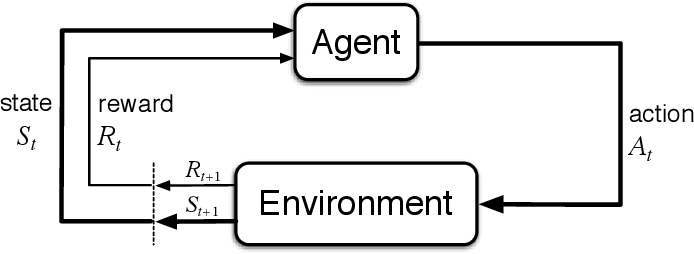
\includegraphics[width=10cm]{figures/background_lit_fig/agent_env_interaction.png}
    \caption{Reinforcement learning model (Source: ~\cite{Sutton1998})}
    \label{fig:reinforcement_learning}
\end{figure}

Q-learning algorithm~\cite{watkins1992q-learning} is a learning method used for estimating the action-value function,
called the Q value, which is the basis for modern reinforcement learning algorithms. The Q value represents the estimated
discounted reward in the future given an action in a particular state. Equation~\eqref{eq:q_value} gives a
mathematically description where rewards in the future are discounted. A recursive version of this equation can be
formulated as equation~\eqref{eq:q_learning} where the next state is the max Q value of the next state-action.

\begin{align}
    Q(s_t, a_t) = E[R_{t+1} + \gamma R_{t+2} + \gamma^2 R_{t+2} + \cdots ] \label{eq:q_value} \\
    Q(s_t, a_t) = Q(s_t, a_t) + \alpha \cdot (r_t + \gamma \cdot \text{max}_a Q(s_{t+1} , a) - Q(s_t, a_t) ) \label{eq:q_learning}
\end{align}

However the curse of dimensionally was found to be a major problem for using Q learning. As it requires a table for
every state-actions pairs so that as the number of state dimensions or actions increased, the table will grow
exponentially. This made the method impractical for problems with large state space due to both the table
size and the required training time.

Therefore function approximators are used to circumvent this problem, typically done using neural networks due to their
ability to approximate any function~\citep{csaji2001approximation} and to be trained using gradient descent.
Work by~\cite{atari}, that implemented a deep convolution neural network achieved state-of-the-art performance in six
of seven games tested as part of the Atari game engine, with three of these scores being superhuman. This was done
through using of two different neural network, a model and target network in which the target network was slowly
updated by the model network to act as a slowly updating target Q value. An experience replay buffer was also
implemented to enable the agent to learn from previous actions.
Follow up work by~\cite{mnih2015humanlevel} found that with no modifications to the hyperparameters, neural network or
training method; state-of-the-art results were achieved in almost all 49 Atari games with superhuman results in 29 of
these games. The work showed that deep neural networks could be trained through observing just the raw game pixels and
knowledge of the game score over time to achieve scores better than humanly possibly.

Due to this research, a large number of heuristics have been proposed to the loss function~\citep{doubledqn},
network architecture~\citep{duelingdqn}, experience replay buffer~\citep{prioritizedexperiencereplay} and more to
improve the optimality of the agent. A combined agent~\citep{rainbow} applying a range of heuristics enabling it to
achieved over 200\% of the original DQN algorithm in score.

\begin{wrapfigure}{l}{0.5\textwidth}
    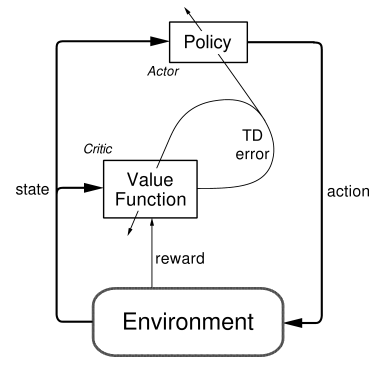
\includegraphics[width=0.5\textwidth]{figures/background_lit_fig/actor-critic.png}
    \caption{Actor Critic model (Source: ~\cite{Sutton1998})}
    \label{fig:actor-critic-model}
\end{wrapfigure}

Using the base of Q-learning, policy gradient agents, shown in figure~\ref{fig:actor-critic-model} separate the action
selection policy from the Q-value function known as the critic. In deep Q networks, actions are selected on the maximum
Q-value for all of the actions, however this requires actions to be discretized. By splitting the actions from the Q
values, an actor chooses an action based on the environment state allowing for both discrete and continuous action space.
With the actor being trained by the value of the critic agent that uses both the state and actor actions to calculate the
Q value for the agent. This has the additional advantage that agents don't require epsilon greedy action selection during
training which can result in the DQN policy differing from the optimal policy. As a result policy gradient has been
used to master the game of Go~\citep{silver2017mastering} and achieve top 1\% in both
Dota 2~\citep{OpenAI_dota} and Starcraft 2~\citep{starcraft2} video games.
%TC:group longtable 0 0

\chapter{Optimising resource allocation in MEC}\label{ch:proposed-solution}
In chapter~\ref{ch:project-problem}, the problem that this project aims to address was outlined along with a short
description of the proposed solution. This chapter builds upon that, giving a formal mathematical model for the problem
in section~\ref{sec:optimisation-problem}. Section~\ref{sec:auctioning-of-tasks} proposes an auction mechanism in order
to pay servers for their resources in order to deal with self-interested users and as server are payed for use of their
services. \\
Using the optimisation problem and auction mechanism from the previous sections, agents for both auction and resource
allocation are proposed, in section~\ref{sec:proposed-agents}, that learns together to maximise a server's profits
over time.

\section{Resource allocation optimisation problem}\label{sec:optimisation-problem}
Using the flexible resource principle, the time taken for a operation to occur, e.g.\ loading of a program, computing
the program and sending of results, etc, is proportional to the amount of resources allocated to complete the operation.
A modified version of a resource allocation optimisation model can be formatted by building upon a similar formulation
in~\cite{FlexibleResourceAllocation}.

A sketch of the whole system is shown in figure~\ref{fig:system_model}.
The system is assumed to contain a set of $I = \{1,2,\ldots,\left|I\right|\}$ servers that are heterogeneous in all
characteristics. Each server has a fixed resource capacity: storage for the code/data needed to run a task
(e.g., measured in GB), computation capacity in terms of CPU cycles per time interval (e.g., measured in GHz),
and communication bandwidth to receive the data and to send back the results of the task after execution
(e.g., measured in Mbit/s). The resources for server $i$ are denoted: $S_i$ for storage capacity, $W_i$ for computation
capacity, and $R_i$ for communication capacity. The system occurs over time that is defined as the set
$T = \{1,2,\ldots,\left|T\right|\}$.

\begin{wrapfigure}{l}{0.5\textwidth}
    \centering
    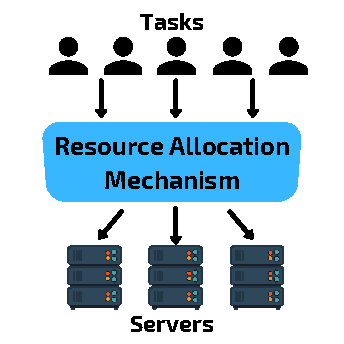
\includegraphics[width=0.5\textwidth]{figures/2_solution_figs/system_model.pdf}
    \caption{System model}
    \label{fig:system_model}
\end{wrapfigure}

The system is also assumed to contain a set of $J = \{1,2,\ldots,\left| J \right|\}$ heterogeneous tasks that require
services from one of the servers in set $I$. To run any of these tasks on a server requires storing the appropriate
code/data on the same server. This could be, for example, a set of images, videos or Convolutional neural network
layers used in identification tasks.\\
The storage size of task $j$ is denoted as $s_j$ with the rate at which the program is transferred to a server at time
$t$ being $s^{'}_{j,t}$. For a task to be computed successfully, it must fetch and execute instructions
on a CPU. We consider the total number of CPU cycles required for the program to be $w_j$, where the number of
CPU cycles assigned to the task at time $t$ is $w^{'}_{j,t}$. Finally, after the task is run and
the results obtained, the latter needs to be sent back to the user. The size of the results for task $j$ is denoted with
$r_j$, and the rate at which they are sent back to the user is $r^{'}_{j,t}$ on a server at time $t$. \\
The allocation of a task to server is denoted by $x_{i,j}$ for each task $j \in J$ and each server $i \in I$. This is
constrained by equation~\eqref{eq:server_task_allocation} meaning that a task can only be allocated to a single server
at any point in time.

\begin{align}
    \sum_{i \in I} x_{i,j} \leq 1 && \forall{j \in J} \label{eq:server_task_allocation} \\
    x_{i,j} \in \{0, 1\} && \forall{i \in I, j \in J} \label{eq:server_task_binary}
\end{align}

As the task must complete each stage in series, additional variables are required to track the progress of
each task stage. $\hat{s}_{j,t}$ denotes the loading progress of the task, $\hat{w}_{j,t}$ denotes the compute progress
and $\hat{r}_{j,t}$ denotes the sending progress of the task. Each of these variables are updated recursively depending
on the progress in the previous time step plus the resources allocated. Progress is also limited to each of the tasks
total required resources in constraints~\eqref{eq:loading_progress_limit},~\eqref{eq:compute_progress_limit}
and~\eqref{eq:sending_progress_limit}.

\begin{align}
    \hat{s}_{j,t+1} = \hat{s}_{j,t} + s^{'}_{j,t} && \forall{j \in J, t \in T } \label{eq:loading_progress} \\
    \hat{w}_{j,t+1} = \hat{w}_{j,t} + w^{'}_{j,t} && \forall{j \in J, t \in T } \label{eq:compute_progress} \\
    \hat{r}_{j,t+1} = \hat{r}_{j,t} + r^{'}_{j,t} && \forall{j \in J, t \in T } \label{eq:sending_progress} \\
    \hat{s}_{j,t} \leq s_j && \forall{j \in J, t \in T} \label{eq:loading_progress_limit} \\
    \hat{w}_{j,t} \leq w_j && \forall{j \in J, t \in T} \label{eq:compute_progress_limit} \\
    \hat{r}_{j,t} \leq r_j && \forall{j \in J, t \in T} \label{eq:sending_progress_limit}
\end{align}

Every task has an auction time, denoted by $a_j$ and a deadline, denoted by $d_j$. This is the time step when the task
is auctioned and the last time for which the task can be completed successfully. During this time, the time required
to send the data/code to the server, run it on the server, and get back the results to the user which must occur in
order. As a server couldn't start computing a task that was already fully loaded on the machine, for example. A
deadline constraint can simply be constructed such that the sending results progress is finished on the deadline
time step (equation~\eqref{eq:deadline}).

\begin{align}
    \hat{r}_{j, d_j} = r_j && \forall{j \in J} \label{eq:deadline}
\end{align}

As servers have limited capacity, the total resource usage for all tasks running on a server must be capped.
The storage constraint (equation~\eqref{eq:server_storage_capacity}) is unique as the sum of the loading progress for
each task allocated to the server. While the computation capacity (equation~\eqref{eq:server_computation_capacity}) is
the sum of compute resources used by all of the tasks on a server $i$ at time $t$ and the bandwidth capacity
(equation~\eqref{eq:server_bandwidth_capacity}) being less than the sum of resources used to load and send results back
by all allocated tasks.

\begin{align}
    \sum_{j \in J} \hat{s}_{j,t} x_{i,j} \leq S_i, && \forall{i \in I, t \in T} \label{eq:server_storage_capacity} \\
    \sum_{j \in J} w^{'}_{j,t} x_{i,j} \leq W_i, && \forall{i \in I, t \in T} \label{eq:server_computation_capacity} \\
    \sum_{j \in J} (s^{'}_{j,t} + r^{'}_{j,t}) x_{i,j} \leq R_i, && \forall{i \in I, t \in T} \label{eq:server_bandwidth_capacity}
\end{align}

\section{Auctioning of Tasks}\label{sec:auctioning-of-tasks}
While the mathematically description of the problem presented in the previous section doesn't consider any auctions
occurring. In real life servers are normally paid for the use of their resources through auctions as discussed in
Section~\ref{sec:resource-allocation-and-pricing-in-cloud-computing}. However due to the modifications
that this project has to make to the optimisation problems, all of the auction mechanisms discussed compatible due to
users not requesting a fixed amount of resources nor can the available resources be easily computed as this is dynamic,
depending on the different stages of tasks allocated to a server. Also the modifications effect the algorithms presented
in~\cite{FlexibleResourceAllocation} as they assume that all of the task stages can occur concurrently. This means that
a novel or modified auction mechanism must be used to deal with these changes. Due to the complexities of devising a new
auction mechanism and the large corpus of research on auctions already, an outline of the most common auctions is
presented in table~\ref{tab:auctions_descriptions} with their respective properties in table~\ref{tab:auction_properties}.

\begin{longtable}{|p{3.5cm}|p{11cm}|} \hline
    \textbf{Auction type} & \textbf{Description} \\ \hline
    English auction & A traditional auction where all participants can bid on a single item with the price slowly
        ascending till only a single participant is left who pays the final bid price. Due to the number of rounds,
        this requires a large amount of communication. \\ \hline

    Dutch auction & The reverse of the English auction, where the starting price is higher than anyone is willing to
        pay with the price slowly dropping till the first participant "jumps in". This can result in sub-optimal pricing
        if the starting price is not high enough or a large number of rounds is required till anyone bids. Plus due
        the auctions occurring over the internet, latency can have a large effect on the winner. \\ \hline

    Japanese auction & Similar to the English auction except that the auction occurs over a set period of time with the
        bid increasing over time and last highest bid being the winner. This means that it has the same disadvantages
        as the English auction except that there is no guarantee that the price will converge to the maximum. Plus
        additional factors like latency can have a large effect on the winner and resulting price. But due to the time
        limit, it has a known amount of time till it finishes unlike the English or Dutch auctions. \\ \hline

    Blind auction & Also known as a First-price sealed-bid auction, all participants submit a single secret bid for an
        item with the highest bid winning. As a result there is no dominant strategy (not incentive compatible) as an
        agent would wish to bid only a small amount more than the next highest price in order overpay for the item.
        But due to there being only a single round of biding, latency doesn't affect an agent and allows many
        more auctions could occur within the same time compared to the English, Dutch or Japanese auctions. \\ \hline

    Vickrey auction~\citep{vickrey} & Also known as a second-price sealed bid auction, participants each submit
        a single secret bid for an item with the highest bid winning like the blind auction. However the winner only
        pays the price of the second highest bid. Because of this, it is a dominant strategy (incentive compatible)
        for an agent to bid its true value as even if the bid is much higher than all other participants its doesn't
        matter as they pay the minimum required for them to win. \\ \hline
    \caption{Descriptions of feasible auctions for the project: English, Dutch, Japanese, Blind and Vickrey auction}
    \label{tab:auctions_descriptions}
\end{longtable}

\begin{table}[h]
    \centering
    \begin{tabular}{|l|c|c|c|} \hline
        \textbf{Auction}  & \textbf{Incentive compatible} & \textbf{Number of rounds} & \textbf{Fixed time length} \\ \hline
        English           & False                         & Multiple                  & False            \\ \hline
        Japanese          & False                         & Multiple                  & True             \\ \hline
        Dutch             & False                         & Multiple                  & False            \\ \hline
        Blind             & False                         & Single                    & True             \\ \hline
        Vickrey           & True                          & Single                    & True             \\ \hline
    \end{tabular}
    \caption{Properties of the auctions described in Table~\ref{tab:auctions_descriptions}}
    \label{tab:auction_properties}
\end{table}

The auction properties that this project considers most important is the auction time length and incentive compatibility.
This is as online auction wish to be fast, making the English, Dutch and Japanese auctions undesirable, and
the incentive compatible properties that means an optimal strategy actually exists. Because of these two
properties, the Vickrey auction~\citep{vickrey} has been chosen. An additional advantage of incentive compatibility,
is that agents don't need to learn how to outbid another agents. They only needs learn to effectively evaluate each task
meaning that reinforcement learning agents could learn through purely self-play.

However a modification must be made to the auction due to servers generate the prices for tasks rather than task
suggesting a price to the servers. Because of this, the auction is reversed, such that the bid with the minimum price
wins the task instead of the maximum price. The auction therefore works by allowing all servers to submit their bids for
a task with the winner being the server with the lowest price, but as this is a Vickrey auction, the server actually
gains second lowest price.

\section{Auction and resource allocation agents}\label{sec:proposed-agents}
Using the optimisation formulation and auction mechanism from the previous two sections, the problem can be modelled as
Markov Decision Process~\citep{Bel} in figure~\ref{fig:mdp_system_model}. This has the advantage of separating out the
auction and resource allocation parts of the problem with separate agents acting for each.
Subsection~\ref{subsec:proposed-auction-agents} and~\ref{subsec:proposed-resource-allocation-agents} proposes agents
for each of the auction and resource allocation environments respectively.

\begin{figure}[h]
    \centering
    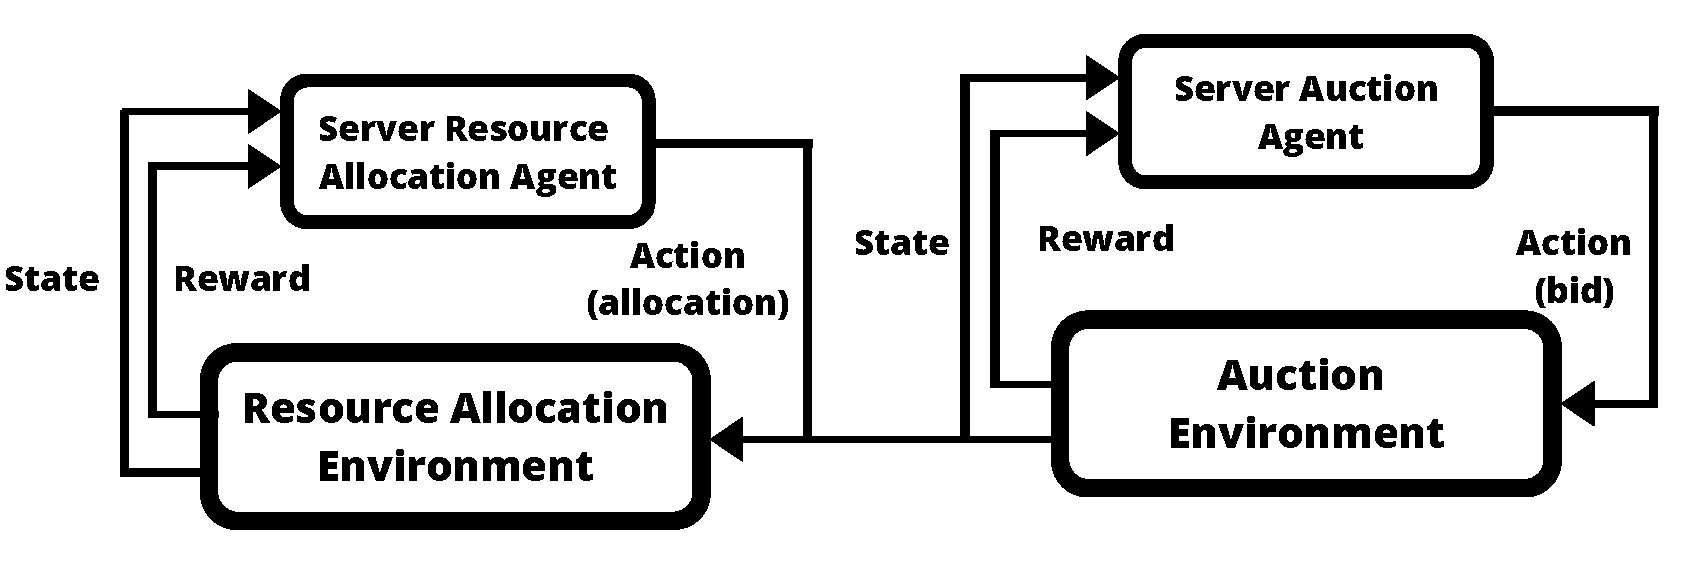
\includegraphics[width=14cm]{figures/2_solution_figs/flexible_resource_allocation_env.pdf}
    \caption{Markov Decision process system model}
    \label{fig:mdp_system_model}
\end{figure}

%The environment is believed to possibly be of interest for multi-agent reinforcement learning researchers as the aim
%of the environment is cooperative (to maximise the social welfare) but knowing that servers can act self-interestedly
%during the auctions in order to maximise their private profits. But the resource allocation agent must work
%cooperatively in allocating of resources for each task as the server wishes to complete as many tasks as they can.
%This author believes that this type of environment is unique within reinforcement learning.

Due to the exploratory nature of the project, a range of reinforcement learning algorithm and neural network
architectures will be implemented and compared to evaluate the effectiveness of each. These are outlined in
Table~\ref{tab:reinforcement_learning_algorithms} for proposed algorithms and Table~\ref{tab:neural_network_layers} for
neural networks.

\begin{longtable}{|p{5cm}|p{10cm}|}
    \textbf{Algorithm} & \textbf{Explanation} \\ \hline
    Dqn~\citep{mnih2015humanlevel} & A standard deep Q learning agent that discretizes the action space with a
        target neural network and experience replay buffer. \\ \hline
    Double Dueling DQN~\citep{doubledqn, duelingdqn} & A combination of two heuristics for the standard deep Q
        learning agents that uses a modified td target function and modified networks that separate the state's value
        and the action advantage. \\ \hline
    Categorical Dqn~\citep{distributional_dqn} & Standard deep Q learning agents return a scalar value
        (representing the q value) for each action. Instead this outputs a probability distribution over action
        values that is helpful for environments that are stochastic. \\ \hline
    Deep deterministic policy gradient~\citep{ddpg} & As the action space is continuous, DDPG allows for
        investigation of the difference between continuous and discrete action spaces of the DQN agents. As policy
        gradient can be more effective at learning a policy where the reward function is too complex for DQN to
        model. \\ \hline
    Twin delay DDPG~\citep{td3} & Like the Double Dueling DQN agents, TD3 includes a couple new heuristics for the
        DDPG algorithm. A critic twin is used to prevent the actor network from tricking the critic network in
        evaluating a state's Q value. Another heuristic is the delaying the updates for actor network compared to the
        critic network to allow the critic to out learn the actor to prevent being tricked.\\ \hline
    \caption{Table of the implemented reinforcement learning algorithms}
    \label{tab:reinforcement_learning_algorithms}
\end{longtable}

\begin{longtable}{|p{3.5cm}|p{10cm}|} \hline
    \textbf{Neural Network} & \textbf{Description} \\ \hline
    Artificial neural networks~\citep{ANN} & Originally developed as a theoretically approximation for the brain, it
        was found that for networks with at least one hidden layer, networks could approximate any
        function~\citep{csaji2001approximation}. This made neural networks extremely helpful for cases where it would
        normally be too difficult for a human to specify the exact function as neural networks can be trained through
        gradient descent to find a close approximation to the true function. \\ \hline

    Recurrent neural network~\citep{RNN} & A major weakness of artificial neural networks is its use of a fixed
        number of inputs and outputs making it unusable with text, sound or video where previous inputs are important
        for understanding a current input. Therefore recurrent neural network's (RNN) extend artificial neural networks
        to allow for connections to previous neurons to "pass on" information. However this was found to struggle from
        vanishing or exploding gradient during training such that gradients would tended either to zero or infinity
        over long sequences. \\ \hline

    Long/Short Term Memory~\citep{LSTM} & While recurrent neural networks can "remember" previous inputs to the
        network, they also struggle from the vanishing or exploding gradient problem. Long/Short Term memory (LSTM) aims
        to remedy this by using forget gates that determine how much information from the last state would get, allowing
        for more complex information to be remembered over time compared to RNNs. \\ \hline

    Gated Recurrent unit~\citep{GRU} & Gated recurrent unit (GRU) are very similar to LSTMs, except for the use of
        different wiring mechanisms with one less gate, an update gate instead of two forget gates. These changes mean
        that GRUs run faster and are easier to code than LSTMs. However are not as expressive meaning that less complex
        functions can be encoded. \\ \hline

    Bidirectional~\citep{Bidirectional} & With RNNs, LSTMs and GRUs, inputs are passed through forward however in
        understanding an input the subsequent inputs are needed. Bidirectional neural network using an inner neural,
        passes in an input twice, once forwards normally and then a second time in reverse. This allows networks to
        understand the context around an input from both before it and after it. \\ \hline

    Neural Turing Machine~\citep{NTM} & Inspired by computers, neural turing machines build on long/short term memory
        by using an external memory module instead of memory being inbuilt to the network. This allows for external
        observers to understand what is going on much better than other networks due to their black-box nature. \\ \hline

    Differentiable neural computer~\citep{DNC} & An expansion to the neural turing machine that allows the memory
        module to be scalable in size allowing for additional memory to be added if needed. \\ \hline

    Sequence to Sequence networks~\cite{seq2seq} & All networks considered above allow for sequences to be passed in
        while outputting an single output vector. Sequence to sequence network utilise two sub-networks; an encoder and
        decoder where the encoder takes a sequence that is encoded into a hidden state that is outputted to the
        decoder that then outputs another sequence. \\ \hline
    \caption{Neural network layer descriptions}
    \label{tab:neural_network_layers}
\end{longtable}

\subsection{Proposed auction agents}\label{subsec:proposed-auction-agents}
Traditionally pricing mechanisms~\citep{al2013cloud} rely on mixture of metrics: resource availability, demand,
quality of service, task resource requirements, task resource allocation quantity, etc to determine a price. However
these values are difficult to approximate during the auction with this program case. So due to the complexity of
deriving this function, reinforcement learning will be used to learn an optimal policy for a server to maximise its
profits over time.

%% TODO Rewrite badly
%As the action space of the agent is continuous, a deep deterministic policy gradient~\citep{ddpg} agent
%will be implemented. The action shape can also be discretized allow deep Q learning agents~\cite{atari} to be trained
%as well. In order to compare alternative learning methods and the affect of discretizing the action space on results,
%agents will use neural networks as it is known to be able to approximate any
%function~\citep{csaji2001approximation}. Because of this, a long/short term memory~\citep{LSTM} layer will be used as
%it allows for multiple inputs, and outputs are single vector that will have several additional layers to allow
%additional complexity. The network will end at a single ReLU neuron for DDPG or multiple logit activation neurons for
%DQN agents as shown in Figure~\ref{fig:task_pricing_network_architecture}.

\begin{figure}
    \centering
    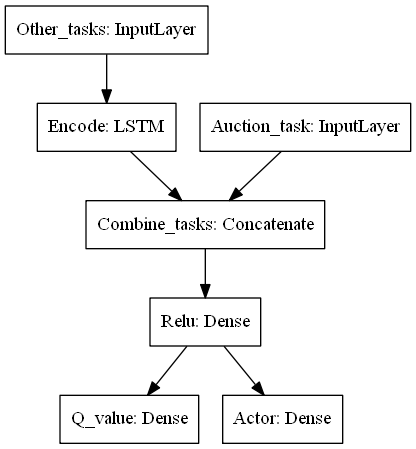
\includegraphics[width=0.5\textwidth]{figures/2_solution_figs/task_pricing_network_architecture.png}
    \caption{Task pricing network architecture}
    \label{fig:task_pricing_network_architecture}
\end{figure}

\subsection{Proposed resource allocation agents}\label{subsec:proposed-resource-allocation-agents}
%% TODO rewrite
When a new task is allocated to the server or a task completes a stage, server resource need to be redistributed
to the task. As the problem of how to allocation resources isn't as complex as the agent pricing in
section~\ref{subsec:proposed-auction-agents}, both simple heuristics and reinforcement learning agents will be
implemented in order to compare effectiveness.

However a similar problem exists as with the proposed auction agents (in subsection~\ref{subsec:proposed-auction-agents}).
Due to knowing how to allocate resources to a single task requires being aware of the resource requirements of other
tasks and how they are being weighted on the server. Therefore a similar network is proposed to allow for the other tasks
to be passed into the network at the same time it is weighting a task. This is shown in
figure~\ref{fig:resource_weighting_network_architecture}

A weighting heuristic is proposed for the network output as well, such that the network doesn't output the raw
resources allocated for a task but rather a weighted value for the resources needing to allocated for the task.
This has the advantage of being a simpler function to approximate for agents but with a similar expressiveness as an
exact resource usage function. This also avoids the problem of the network either over allocating the resources to tasks
or severely under allocating resources.

\begin{figure}
    \centering
    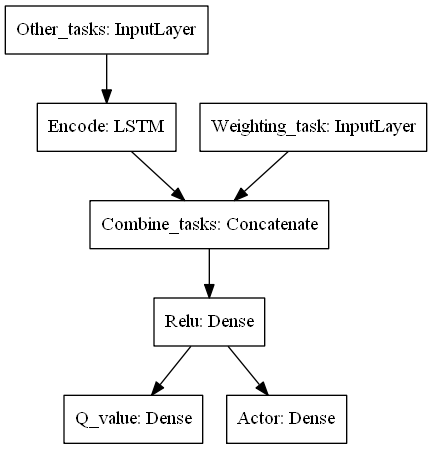
\includegraphics[width=0.5\textwidth]{figures/2_solution_figs/resource_weighting_network_architecture.png}
    \caption{Resource weighting network architecture}
    \label{fig:resource_weighting_network_architecture}
\end{figure}



% For the listing caption reference
%! Suppress = UnresolvedReference

% To ignore word count of agent hyperparameters
%TC:group longtable 0 0

\chapter{Implementing a flexible resource allocation environment and agents}\label{ch:implementation-of-the-solution}
In order to implement a solution from chapter~\ref{ch:proposed-solution}, an MEC network environment
must be simulated due to the impractically of setting up such a network and in order to train the agents offline as
proposed in section~\ref{sec:proposed-agents}. This chapter splits the implementation into three sections: the
environment simulation (section~\ref{sec:simulating-edge-cloud-computing-services}), server auction and resource
allocation agents (section~\ref{sec:implementing-auction-and-resource-allocation-agents}) and training of agents
(section~\ref{sec:training-agents}).

The implementation discussed below as written in Python and available to download from
Github~\footnote{\url{https://github.com/stringtheorys/Online-Flexible-Resource-Allocation}}. The reason for the use of
python is number of modules available for reinforcement learning and the speed of development.

\section{Simulating edge cloud computing services}\label{sec:simulating-edge-cloud-computing-services}
While the aim of the environment is the simulate accurately MEC servers, the implementation of the environment must
allow agents to train on interact and training on the environment efficiently. Therefore it has been implemented
as an OpenAI gym~\citep{openaigym}, the de facto standard for implementing reinforcement learning environment for
researchers. However the standard specification must be modified due to the problem being multi-agent and multi-step.

An example for running the environment is in listing~\ref{lst:example_flexible_resource_env}. There are three
sections to the code: the first is the construct an environment using the constructor, where the environment settings
are passed that determines the number of servers, tasks and their attributes. These attributes are determined using
uniform random numbers between a maximum and minimum values that are synthetically generated for each variable. The
second step is to create the environment using the reset function returning the new environment state. The environment
state contains a task if one needs to be auctioned and a dictionary of server to their current task state. Using these
states, each server can generate actions either using the auction agent or resource allocation agent depending if a task
needs auctioning. The final part is to take a step using the server actions that returns an updated server state, the
rewards for the actions, if the environment is finished and an extra information from the steps taken. The rewards is a
dictionary of each of servers with either the winning price for the auctioned task or a list of tasks that have
finished either because they ran out of time or completed the task early, depending on the step taken.

\begin{lstlisting}[language=Python, frame=single, caption={Example code for running the environment}, captionpos=b, label={lst:example_flexible_resource_env}]
# Load the environment with a setting
env = OnlineFlexibleResourceAllocationEnv('settings.env')

# Generate the environment state
server_state = env.reset()

for _ in range(1000):
    # Generate actions
    if server_state.auction_task:
        actions = {
            server: auction_agent.bid(state)
            for server, state in server_state
        }
    else:
        actions = {
            server: resource_allocation_agent.weights(state)
            for server, state in server_state
        }

    # Take environment step
    server_state, reward, done, info = env.step(actions)

    # If the environment is finished then reset it
    if done:
        server_state = env.reset()
\end{lstlisting}

\subsection{Weighted server resource allocation}\label{subsec:weighted-server-resource-allocation}
A particular complication of the environment is to distribute server resources due to the fact that the resource
allocation agents provide a resource weighting rather than the actually task resource usage. Because of this, a novel
algorithm was implemented to convert the weighting to actual resources for each task.

To allocate the computational resources is relatively simple compared to allocating resources for both storage and
bandwidth. For computational resources, the algorithm checks first if the weighted resources is greater than the
quantity required for the task to finish the compute stage of a task. If this is true then a resources needed for the
task to complete the compute stage are allocated. However, this also means that the weight resources available for each
task is increased due to a task not using all of the resources it could. This type of checking is repeated till no task
can be finished with its weighted resource within this time step. For the remaining task, they are just allocated their
weighted compute resources.

For allocating storage and bandwidth, this is more difficult is due to the fact that when the server is still
loading the task, the server is allocating both storage and bandwidth resources while also allocating bandwidth
resources to tasks sending results back to users. Because of this, a tension exists between allocating bandwidth and
storage resources for all of the tasks fairly. Algorithm was therefore chosen to gives priority when allocating
resources to the tasks sending results as these tasks are more likely to be finished and aims to not penalise the
server for not completing the task within the deadline.

To allocate resources, a similar function to used to the one for allocating compute resources. First a check if done
using the weighted bandwidth resources to see if any task sending results will be finished with the resources.
This process is also repeated for the tasks loaded onto a server with the additional check that there is enough
available storage for the new data to be added. For any remaining task, this process is repeated till all of the
available resources are allocated in the time step. As a results, using this algorithm, the converting between
weightings to resources allowing for allocating of almost all of the server's resources with no resources unused.

\section{Implementing Auction and resource allocation agents}\label{sec:implementing-auction-and-resource-allocation-agents}
To implement auction and resource allocation agents, generic abstract classes for both were implemented with a bid
function for the auction agent and a weighting function for the resource weighting agent. The bid had arguments for the
task being auctioned, the server with its currently allocated tasks and current time step. These attribute were used by
the reinforcement learning policies explained in subsection~\ref{subsec:implementing-auction-and-resource-allocation-agents}
to calculate the auction bid price. For the weighting function in the resource weighting agent, the function took a
server and a list of the server's currently allocated tasks along with the current time step. Using these attributes,
agents can return a dictionary of task weighting.

A range of different reinforcement learning techniques have been implemented, outlined in
Table~\ref{tab:reinforcement_learning_algorithms}, in order to explore the different options that a server would have
available to learn its policies.

\subsection{Implementing reinforcement learning policies}\label{subsec:implementing-auction-and-resource-allocation-agents}
The policies outlined in table~\ref{tab:reinforcement_learning_algorithms} were implemented using
tensorflow~\citep{tensorflow2015-whitepaper}, a python module developed by Google
that provides programmers the ability to construct neural network, backpropagation with custom loss function and more.
For each of the algorithms, an abstract class was implemented with a function for training and saving of the agent
neural networks. For each of these algorithms, a task pricing and resource weighting class was implemented that are
subclasses for the abstract algorithm class.

Both deep Q networks and policy gradient algorithm are based on the Q function (explained in
section~\ref{sec:reinforcement-learning})) which tries to approximate the reward at the next time step. To do
this requires a reward function and a next observation to compare to in order to train these agents. The agent's
reward function and agent training observations are detailed in subsection~\ref{subsec:agent-rewards-functions}
and~\ref{subsec:agent-training-observations}.

\begin{table}
    \centering
    \begin{tabular}{|p{5cm}|p{10cm}|} \hline
        Policy Type & Explanation \\ \hline
        Dqn~\citep{mnih2015humanlevel} & A standard deep Q learning agent that discretizes the action space with a
            target neural network and experience replay buffer. \\ \hline
        Double Dueling DQN~\citep{doubledqn, duelingdqn} & A combination of two heuristics for the standard deep Q
            learning agents that uses a modified td target function and a modified networks that separates state value
            and action advantage which can recombined at the end. \\ \hline
        Categorical Dqn~\citep{distributional_dqn} & Standard deep Q learning agents return a scalar value
            (representing the q value) for each action. Instead this outputs a probability distribution over action
            values that is believed to be helpful due to the stochastic nature from the problem (from the agents
            perspective). \\ \hline
        Deep deterministic policy gradient~\citep{ddpg} & As the action space is continuous, DDPG allows for
            investigation of the difference between continuous and discrete action spaces of the DQN agents. As policy
            gradient can be more effective at learning a policy where the reward function is too complex for DQN to
            model this may give the algorithm another advantage. \\ \hline
        Twin delay DDPG~\citep{td3} & Like the Double Dueling DQN agents, TD3 includes a couple new heuristics for the
            DDPG algorithm. A critic twin is used to prevent the actor network from tricking the critic network, another
            heuristic is the delaying the updates for actor network compared to the critic network.\\ \hline
        D4PG~\citep{d4pg} & Like the Categorical DQN algorithm, D4PG adds a heuristic for the critic to output a
            value distribution that allows for better approximation for environments that are stochastic in nature.
            \\ \hline
    \end{tabular}
    \caption{Table of the implemented reinforcement learning algorithms}
    \label{tab:reinforcement_learning_algorithms}
\end{table}

A particular problem that this project encounter was with using recurrent neural network as inputs. This is as the
number of inputs is not fixed meaning that during training, using a minibatch was not possible as most of the inputs
all had different input lengths and tensorflow requires all inputs to have a known, fixed length. Originally this was
sidestepped by calculating the loss for each input individually then finding the mean loss and gradient to update the
networks with. However this was found to be computationally impractical making the method impossible to run agents to
long enough. Because of this, a solution was found by padding all of the inputs to have the same size using the
tensorflow preprocessing module with the sequence.pad\_sequence function. As a result, training became ~10x faster
making large scale testing practical.

\subsection{Agent rewards functions}\label{subsec:agent-rewards-functions}
As explained in the background review for reinforcement learning (section~\ref{sec:reinforcement-learning}),
the Q values is the estimated discounted reward in the future for an action given a particular state. Therefore the
rewards that an agent receives for taking an action is extremely important to enable the agent to learn a predictable
reward function. This problem of complex reward functions are a known problem for DQN agent to deal with~\citep{atari}m
policy gradients can deal with this better due its ability directly learning the action policy~\citep{Sutton1998}.

For the auction, the reward is based on the winning price of the task which is award for the winning action. If the
task fails, the reward is instead multiplied by a negative constant in order to discourage the auction agent from
bidding on tasks that it wouldn't be able to complete. This reward is awarded at the time step of the auction instead of
when the task fails or is completed as this makes the function harder to learn as the auction agent has no control or
observations over the resource allocation for a task. \\
As the price of zero is treated as a non-bid in the auction, the agent gets a reward of zero in order to not
penalise the agent. But if the agent does bid on a task however doesn't win, the agent's reward is -0.05 as a way of
encouraging the agent to change there bid but not enough to force it to do so.

For resource allocation, the reward function is much simpler than the auction agent's reward function, as it only needs
to consider the task being weighted at the time and rewards from other tasks allocated at the same time step. This is
as a task must consider its actions in conjunction with the resource requirements of other allocated tasks. \\
For successfully finishing a task, the reward is 1 while the reward for if the task has failed is -1.5. This makes
failing a task more costly than completing a task. But when a task's action is not under consideration, this reward is
multiplied by 0.4 as while this rewards impact the task, their value is not as impactful as the reward for the action
on a particular task. These rewards don't consider the price payed for the task instead valuing each task equally with
the aim of forcing the task allocate resources to finish all tasks not just the valuable ones. Using this information,
the reward function is simply the sums the rewards of the finished tasks in the next time step.

\subsection{Agent training observations}\label{subsec:agent-training-observations}
As the agent acts in the environment, the observations that the agent views are stored in an experience replay buffer
which allows the agents to train from previous observations. However this is a problem for agent due to the separate
agents acting with only during its particular action step. This is outlined in figure~\ref{fig:environment-observations},
where an agents next observation is often after subsequent actions by the opposite agent.

\begin{figure}
    \centering
    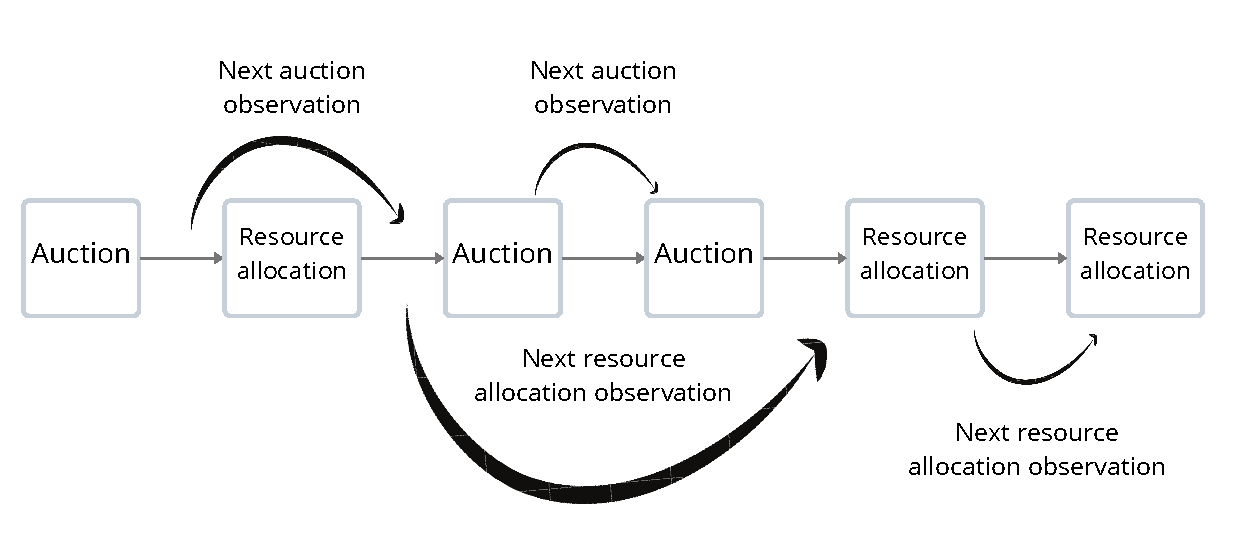
\includegraphics[width=14cm]{figures/implementation_fig/env_server_agents_observations.pdf}
    \caption{Environment server agents observations}
    \label{fig:environment-observations}
\end{figure}

For the resource allocation agent, a trick is implemented such that the next observation for the agent is not the
actual next resource allocation observation as shown in figure~\ref{fig:environment-observations} but a generated
observation from the resulting server state due to agent's actions. This is identical to the last case in the figure
where no auction occurs between resource allocation steps. Because of this, the resource allocation Q value is able to
approximate the reward for the results state of its actions directly making it appear to the agent during training that
there is no auction steps between the observations and next observations.
% Todo add number of tasks observations problems

For the auction agent, as the agent observations require an auction task to select an action (the task bidding price).
A trick like the one implemented for the resource allocation agent can't be to implement. Therefore during training,
each server's last observation is recorded, such that when the next auction occurs, this new task observation can be
used as the server's next observation in training. This is a suboptimal solution for the agent as the next observation
has an unknown number of resource allocation steps resulting in changes to the current allocated tasks.
A possible solution that has not been implement in this project is n step prediction~\citep{multi-step-dqn}. Where the
agent doesn't predict the Q value of the next environment, but the value in n steps time. This is believed to possible
help reduce the amount of randomness in the server's observations and improve bidding performance.

\section{Training agents}\label{sec:training-agents}
The first section of this chapter allowed for the simulating MEC servers
(section~\ref{sec:simulating-edge-cloud-computing-services}) as a reinforcement learning environment. While the second
section implements auction and resource allocation agents that can interact with the porpoised environment in order
to allow for the train of agents using a range of algorithm outlined in Table~\ref{tab:reinforcement_learning_algorithms}.

Neural networks, the bases of the reinforcement learning agents implemented, often require huge amounts of data and
high spec GPUs to run efficiently. Because of this, Iridis 5, University of Southampton supercomputer was utilised with
GTX1050 GPUs to train these agents for long periods of time and on mass. During training, for each episode a random
environment was generated from a list of possible settings in which the agents would be allocated to random servers. The
environment was run till the end, with the agent observation being added to their replay buffers after each actions
that were chosen epsilon greedily.

After every 5 episodes, the agents would be evaluated using a set of environment that were pre-generated and
saved at the beginning of training. This allows the same environments over training in order to have a constant metric
in order to compare the agents over time. The actions taken are recorded to be used in evaluation
(chapter~\ref{ch:evaluation-of-the-solution}) with the number of completed and failed tasks being stored about
the resource allocation agent and the winning prices being stored about the auction agents. Plus an action histograms
for each agents in order to view how agents bid and weightings are distributed.

\subsection{Agent training hyperparameters}\label{subsec:agent-training-hyperparameters}
During training there are a range of hyperparameters for each agent, table~\ref{tab:agent_hyperparameters} provides
an explanation of value for all of the hyperparameters used in the project.

\begin{longtable}{|p{2cm}|p{3.5cm}|p{2.5cm}|p{6cm}|} \hline
    \textbf{Agent} & \textbf{Properties name} & \textbf{Value} & \textbf{Explanation} \\ \hline
        RL Agent & batch\_size & 32 & The number of trajectories from the experience replay buffer that are used each
            time to train an agent. \\ \hline
        RL Agent & error\_loss\_fn & tf.losses. huber\_loss & The loss function for calculating the error that similar
            the mean squared loss exact has a smaller gradient. \\ \hline
        RL Agent & initial\_training replay\_size & 5000 & The number of trajectories in the experience replay buffer
            required before the agent begins training. \\ \hline
        RL Agent & training\_freq & 2 & For every trajectory added to the experience replay buffer, for each 2, the
            agent tries to be trained. \\ \hline
        RL Agent & discount\_factor & 0.9 & Within the Q learning function (equation~\eqref{eq:q_learning}), the
            discount factor determines how important the rewards in the future impact the Q value. \\ \hline
        RL Agent & replay\_buffer length & 25000 & The length of the circular experience replay buffer. \\ \hline
        RL Agent & save\_frequency & 25000 & The agent networks are saved after 25000 time that agent has been trained
            \\ \hline
        RL Agent & training\_loss log\_freq & 250 & Tensorboard allows for data to be saved using training, after every
            the agent has been trained 250 time, the agents loss is logged for future analysis. \\ \hline
        Task Pricing RL Agent & reward\_scaling & 1 & \\ \hline
        Task Pricing RL Agent & failed\_auction reward & -0.05 & The reward for when the agent bids on a task but fails
            to win the auctioned task. \\ \hline
        Task Pricing RL Agent & failed\_multiplier & -1.5 & A multiplier applied to the winning price is the task fails
            to be computed within its deadline. \\ \hline
        Resource weighting RL Agent & other\_task\_discount & 0.4 & The multiplier to tasks not under consideration for
            a weighting action. \\ \hline
        Resource weighting RL Agent & success\_reward & 1 & The reward when the agent successfully completes a task
            \\ \hline
        Resource weighting RL Agent & failed\_reward & -1.5 & The reward when the agent fails to complete a task within
            its deadline. \\ \hline
        Dqn Agent & target\_update\_tau & 1.0 & The update tau value for use in the target update frequency. \\ \hline
        Dqn Agent & target\_update\_freq & 2500 & The target network in the DQN agent is updated after the agent
            has been updated 2500 times. \\ \hline
        Dqn Agent & initial\_epsilon & 1 & The initial exploration factor during training \\ \hline
        Dqn Agent & final\_epsilon & 0.1 & The final exploration factor during training \\ \hline
        Dqn Agent & epsilon\_steps & 10000 & The number of training step for linear exploration to move between the
            initial\_epsilon and the final\_epsilon factor. \\ \hline
        Dueling Dqn Agent & double\_loss & True & If to use the double dqn loss function \\ \hline
        Categorical Dqn Agent & max\_value & -20.0 & The maximum value for the value distribution \\ \hline
        Categorical Dqn Agent & min\_value & 25.0 & The minimum value for the value distribution \\ \hline
        Categorical Dqn Agent & num\_atoms & 21 & The number of atoms for each actions. \\ \hline
        Ddpg Agent & actor\_learning\_rate & 0.0001 & The learning rate for the optimiser for the actor network. \\ \hline
        Ddpg Agent & critic\_learning\_rate & 0.0005 & The learning rate for the optimiser for the critic network. \\ \hline
        Ddpg Agent & initial\_epsilon\_std & 0.8 & The initial exploration standard deviation of the normal distribution
            used  during training \\ \hline
        Ddpg Agent & final\_epsilon\_std & 0.05 & The final exploration standard deviation of the normal distribution
            used  during training \\ \hline
        Ddpg Agent & actor\_target update\_freq & 3000 & The actor target network update frequency \\ \hline
        Ddpg Agent & critic\_target update\_freq & 1500 & The critic target network update frequency \\ \hline
        Ddpg Agent & upper\_action bound & 30.0 & The upper action bound for the actor network \\ \hline
        Task pricing Ddpg Agent & min\_value & -100.0 & The minimum value for the critic network to estimate for an
            action \\ \hline
        Task pricing Ddpg Agent & max\_value & 100.0 & The maximum value for the critic network to estimate for an
            action\\ \hline
        Resource allocation Ddpg Agent & min\_value & -20 & The minimum value for the critic network to estimate for an
            action \\ \hline
        Resource allocation Ddpg Agent & max\_value & 15 & The maximum value for the critic network to estimate for an
            action\\ \hline
        TD3 Agent & actor\_update\_freq & 3 & The actor network update frequency for each critic network update. \\ \hline
    \caption{Agent hyperparameters}
    \label{tab:agent_hyperparameters}
\end{longtable}



% Texcount ignores the longtables
%TC:group longtable 0 0

\chapter{Testing and evaluation}\label{ch:testing-and-evaluation}
Using the implemented solution from Chapter~\ref{ch:implementation-of-the-solution} to test and evaluate its
effectiveness, both functional unit tests and agent training evaluation have been designed. To confirm that the
environment and agents implemented in the previous chapter
(section~\ref{sec:implementing-auction-and-resource-allocation-agents}) works as intended, unit testing has been added
that is explained in Section~\ref{sec:functional-testing}. While to evaluate the effectiveness of the proposed
solution from Section~\ref{sec:proposed-agents}, a range of metric have been measured during training in order to
test and compare implemented agents, neural network architectures and training parameters. These results are explained
in Section~\ref{sec:agent-evaluation}.

\section{Functional testing}\label{sec:functional-testing}
To confirm that the implementation of the agents and environment correctly, PyTest a module within python has been used
to design functions are valid. These tests are split into three families: agent, environment and training that are
explained in the respective tables~\ref{tab:agent_testing},~\ref{tab:env_testing} and~\ref{tab:training_testing}.
The results from the testing is shown in figure~\ref{fig:pytest_results}.

\begin{longtable}{|p{3cm}|p{11cm}|} \hline
    \textbf{Testing name} & \textbf{Explanation} \\ \hline
    Building agents & Constructs all of the agents with possible arguments to confirm agents can accept of all its
        attributes\\ \hline
    Saving agents & Confirms that agents can successfully save their neural networks and can successfully load
        the network again and is equal to the agent network. \\ \hline
    Agent actions & Confirms that all agents can generate valid actions for both bidding and weighting \\ \hline
    Gin config file & Gin is used to set the arguments used during training, to confirm that the file is valid. \\ \hline
    Building networks & Constructs all of the neural networks to confirm that the network return a valid output. \\ \hline
    Agent epsilon policy & While training, some of the agent actions are randomly selected to train the agents over
        a large area of the state. This tests that the random actions selected are valid. \\ \hline
    \caption{Table of testing functions for the agent}
    \label{tab:agent_testing}
\end{longtable}

\begin{longtable}{|p{3cm}|p{11cm}|} \hline
    \textbf{Testing name} & \textbf{Explanation} \\ \hline
    Saving and loading an environment & The environment allows for the saving the environment at its current
        state. This tests that the environment can save and reload the environment successfully. \\ \hline
    Loading environment settings & Tests that the load environment settings correctly generates a new random
        environment based on the settings. \\ \hline
    Random action environment steps & To tests that inputs to the auction and resource allocation steps are valid,
        random actions are generated for the environment, that is repeated for the whole environment.  \\ \hline
    Auction step & To confirm the Vickrey auction mechanism is completely implemented, a range of possible inputs
        are tested to confirm that right price and server the task is allocated to. \\ \hline
    Resource allocation step & To confirm that servers allocate their resources correct given some inputs. \\ \hline
    Allocation of computational resources & Checks that the server correctly allocates computational resources to
        allocated tasks. \\ \hline
    Allocation of storage and bandwidth resources & Checks that the server correctly allocates storage and
        bandwidth resources to allocated tasks. \\ \hline
    Allocation of all resources & Checks that resources are allocated by the server correctly for all of the
        resources. \\ \hline
    \caption{Table of testing functions for the environment}
    \label{tab:env_testing}
\end{longtable}

\begin{longtable}{|p{3cm}|p{11cm}|} \hline
    \textbf{Testing name} & \textbf{Explanation} \\ \hline
    Task pricing training & Tests that the task pricing reinforcement learning agents can correctly learning from
        different auction observations. \\ \hline
    Resource allocation training & Tests that resource allocation reinforcement learning agents can correctly
        learning from different resource allocation observations. \\ \hline
    Agent evaluation & Tests that the agent evaluation function for during training correctly captures the correct
        information due to the actions taken. \\ \hline
    Agent training & Tests that agents can be correctly trained over an environment with different actions and
        observations. \\ \hline
    Random actions training & Tests that agents with random actions that can quickly using the environment training
        methods to confirm that the function work as intended. \\ \hline
    \caption{Table of testing functions for agent training}
    \label{tab:training_testing}
\end{longtable}

\begin{figure}[h]
    \centering
    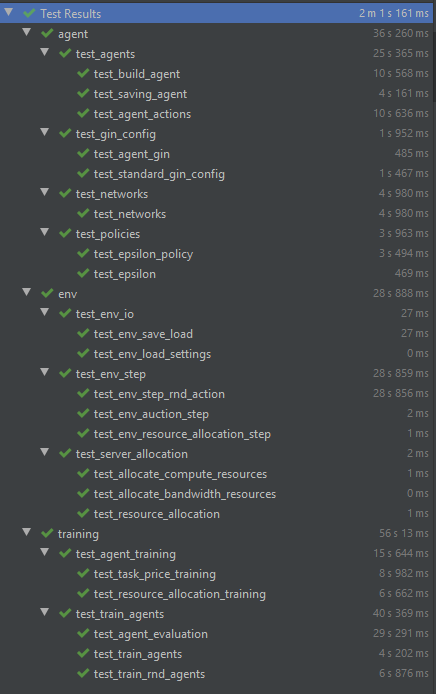
\includegraphics{figures/4_test_eval_figs/pytest_results.PNG}
    \caption{Results of the unit functions described in the Tables~\ref{tab:agent_testing},~\ref{tab:env_testing}
        and~\ref{tab:training_testing}}
    \label{fig:pytest_results}
\end{figure}

\section{Agent evaluation}\label{sec:agent-evaluation}
In order to compare the implemented agents from Chapter~\ref{ch:implementation-of-the-solution}, a range of metric are
used which are recorded while the agent is training. For the auction agent the metrics are: histogram winning prices,
number of no bids, number of failed tasks, number of completed tasks and a histogram of actions taken. For the resource
allocation agents the metrics are a histogram of weighting, number of failed tasks and number of completed tasks.
Using these metrics evaluation of agent performance can be done between the different reinforcement learning algorithms
implemented in Table~\ref{tab:reinforcement_learning_algorithms}, network architectures in
Table~\ref{tab:neural_network_layers} and methods of training different agents. \\
These evaluations fall into three families: env and agent num, algorithm and network architecture that are analysed in
Subsections~\ref{subsec:environment-and-agent-number-training},~\ref{subsec:reinforcement-learning-algorithm-training}
and~\ref{subsec:neural-network-architecture-training} respectively.

\subsection{Environment and Agent number training}\label{subsec:environment-and-agent-number-training}
The analysis of the different reinforcement learning algorithms and neural network architectures in
Subsection~\ref{subsec:reinforcement-learning-algorithm-training} and~\ref{subsec:neural-network-architecture-training}
respectively assume two qualities that this subsection analyses. These are the training and evaluation environments
and the number of agents used during training. As there are huge ranges of possible environment settings that agents
could be trained, investigating agent environment generality is a challenge and an important measure within machine
learning. This is of particular importance for this work, as in real-life, the environment that agents experiences will
can be unpredictable and different from those trained on. Meaning that agents should learn to generalise and not
overfit to particular environments used during training.

The other assume quality is due an advantage of the Vickrey auction over alternative auctions, explored in
Section~\ref{sec:auctioning-of-tasks}, that it is Incentive compatible. This auction property means that the dominant
strategy for all agents is to bid truthfully, which is the agent's true evaluation of the task. Therefore due to agents
not needing to learn to "out bid" each other allowing for effective self-play to be used in training.

Therefore this subsection compare the results of agents that are trained on a single environment setting and those
trained on multiple environment settings and when multiple or single agents are trained together.
These are compared using a set of pre-generated environments, one from the single environment setting and another from
the multiple environment settings.


%% Env training legend
\begin{wrapfigure}{r}{0.5\textwidth}
    \includegraphics[width=0.5\textwidth]{figures/4_test_eval_figs/env_training_fig/legend.png}
    \caption{Environment training legend}
    \label{fig:env-training-legend}
\end{wrapfigure}

During train, every 10 episodes, the agents are trained on the environments pre-generated from the multi-env settings.
Then in each of these evaluations, five metrics are collected: the number of completed tasks
(figure~\ref{fig:env_num_completed_tasks}), number of failed tasks (figure~\ref{fig:env_num_failed_tasks}),
the percentage of tasks attempted (figure~\ref{fig:env_percent_tasks}), total prices (figure~\ref{fig:env_total_prices})
and total winning prices (figure~\ref{fig:env_winning_prices}) when the environment are run.

%% Training evaluation
\begin{figure}[h]
    \centering
    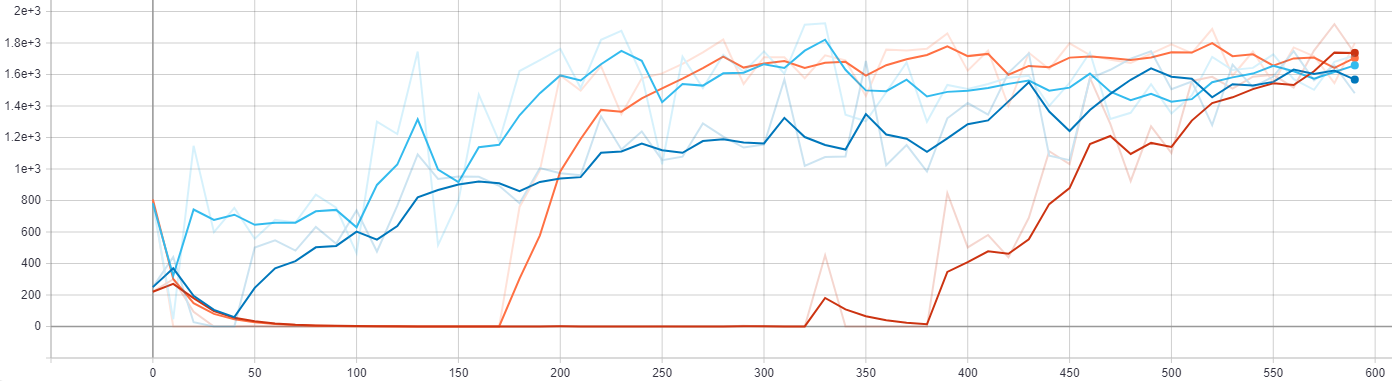
\includegraphics[width=17cm]{figures/4_test_eval_figs/env_training_fig/num_completed_tasks.png}
    \caption{Number of completed tasks}
    \label{fig:env_num_completed_tasks}
\end{figure}

\begin{figure}[h]
    \centering
    \includegraphics[width=17cm]{figures/4_test_eval_figs/env_training_fig/num_failed_tasks.png}
    \caption{Number of failed tasks}
    \label{fig:env_num_failed_tasks}
\end{figure}

\begin{figure}[h]
    \centering
    \includegraphics[width=17cm]{figures/4_test_eval_figs/env_training_fig/percent_tasks.png}
    \caption{Percentage of tasks attempted}
    \label{fig:env_percent_tasks}
\end{figure}

\begin{figure}[h]
    \centering
    \includegraphics[width=17cm]{figures/4_test_eval_figs/env_training_fig/total_prices.png}
    \caption{Total prices}
    \label{fig:env_total_prices}
\end{figure}

\begin{figure}[h]
    \centering
    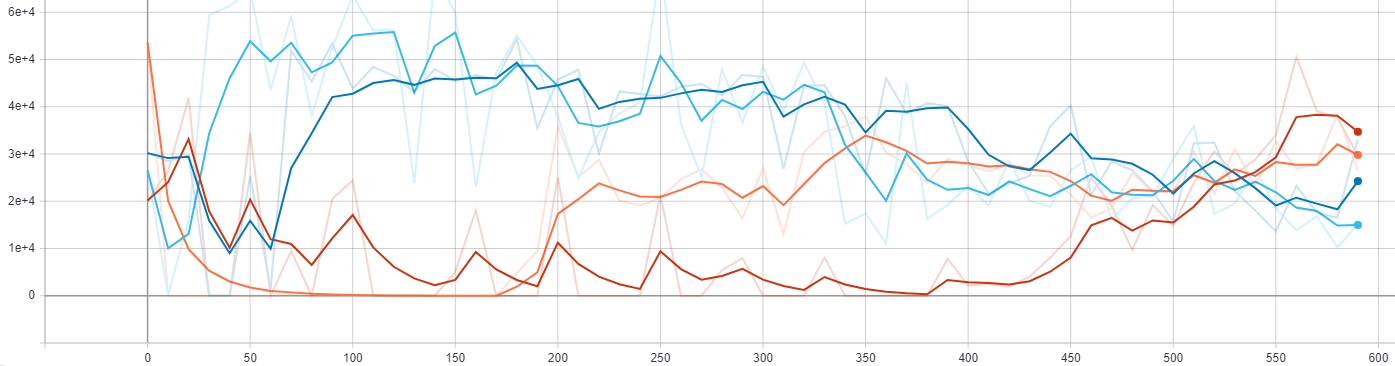
\includegraphics[width=17cm]{figures/4_test_eval_figs/env_training_fig/total_winning_prices.PNG}
    \caption{Total winning prices}
    \label{fig:env_winning_prices}
\end{figure}

%% Analysis of the training results
%% TODO

%% Auction prices and resource weightings histograms
%% TODO
\begin{figure}[h]
    \centering
    \begin{minipage}{0.5\textwidth}
        \centering
        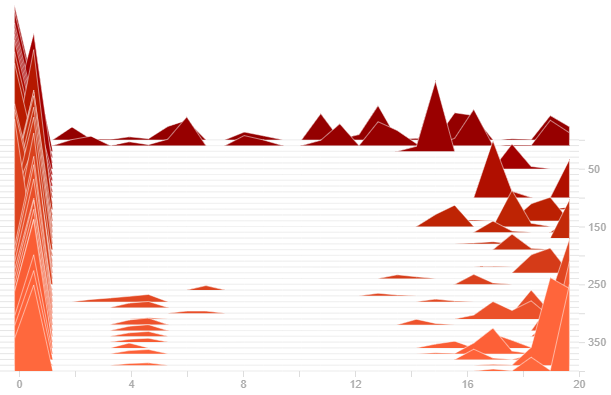
\includegraphics[width=1.0\textwidth]{figures/4_test_eval_figs/env_training_fig/multi_agent_single_env_auction_price.png}
        \caption{Multi agent single environment auction prices}
        \label{fig:multi_agent_single_env_auction_prices}
    \end{minipage}\hfill
    \begin{minipage}{0.5\textwidth}
        \centering
        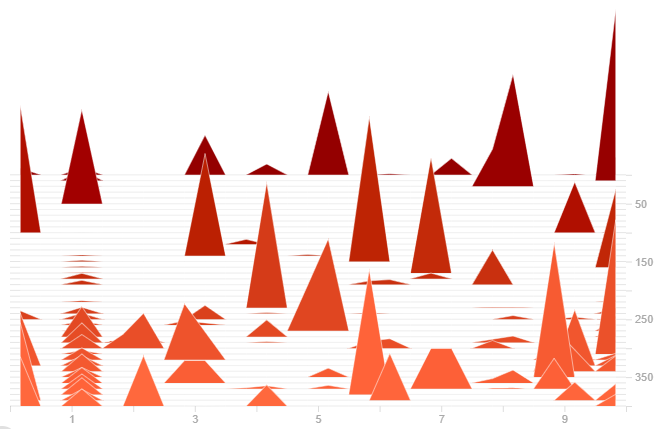
\includegraphics[width=1.0\textwidth]{figures/4_test_eval_figs/env_training_fig/multi_agents_single_env_weightings.png}
        \caption{Multiple agent single environment resource weightings}
        \label{fig:multi_agent_single_env_weightings}
    \end{minipage}
\end{figure}
\begin{figure}[h]
    \centering
    \begin{minipage}{0.5\textwidth}
        \centering
        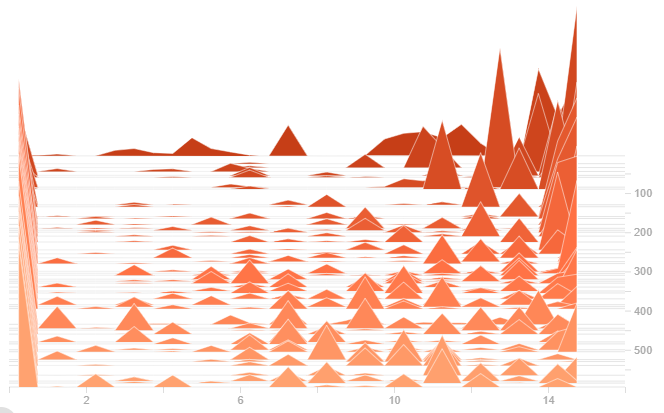
\includegraphics[width=1.0\textwidth]{figures/4_test_eval_figs/env_training_fig/multi_agents_multi_envs_auction_prices.png}
        \caption{Multi agent multi environment auction prices}
        \label{fig:multi_agent_multi_env_auction_prices}
    \end{minipage}\hfill
    \begin{minipage}{0.5\textwidth}
        \centering
        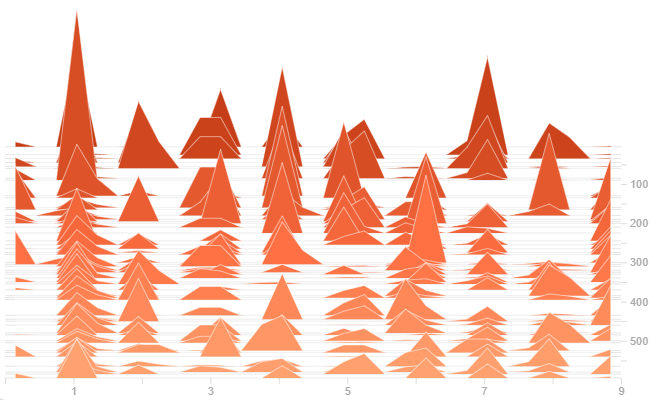
\includegraphics[width=1.0\textwidth]{figures/4_test_eval_figs/env_training_fig/multi_agents_multi_envs_weightings.png}
        \caption{Multiple agent multi environment resource weightings}
        \label{fig:multi_agent_multi_env_weightings}
    \end{minipage}
\end{figure}
\begin{figure}[h]
    \centering
    \begin{minipage}{0.5\textwidth}
        \centering
        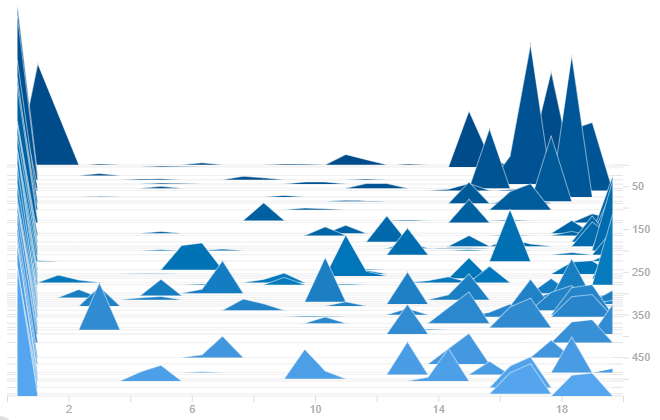
\includegraphics[width=1.0\textwidth]{figures/4_test_eval_figs/env_training_fig/single_agent_single_env_auction_price.png}
        \caption{Single agent single environment auction prices}
        \label{fig:single_agent_single_env_auction_prices}
    \end{minipage}\hfill
    \begin{minipage}{0.5\textwidth}
        \centering
        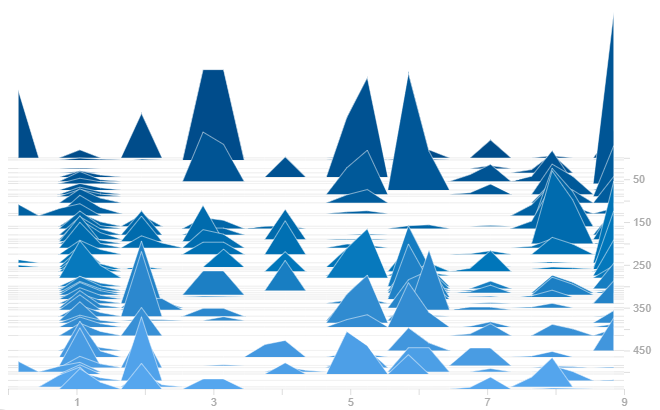
\includegraphics[width=1.0\textwidth]{figures/4_test_eval_figs/env_training_fig/single_agent_single_env_weightings.png}
        \caption{Multiple agent multi environment resource weightings}
        \label{fig:single_agent_single_env_resource_weightings}
    \end{minipage}
\end{figure}

\subsection{Reinforcement learning algorithm training}\label{subsec:reinforcement-learning-algorithm-training}
In table~\ref{tab:reinforcement_learning_algorithms}, a range of reinforcement learning algorithms were proposed as
methods of training neural networks.

\begin{wrapfigure}{l}{0.5\textwidth}
    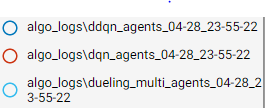
\includegraphics[width=0.5\textwidth]{figures/4_test_eval_figs/algo_training_fig/legend.PNG}
    \caption{Environment training legend}
    \label{fig:algo-training-legend}
\end{wrapfigure}

%% Training evaluation
\begin{figure}[h]
    \centering
    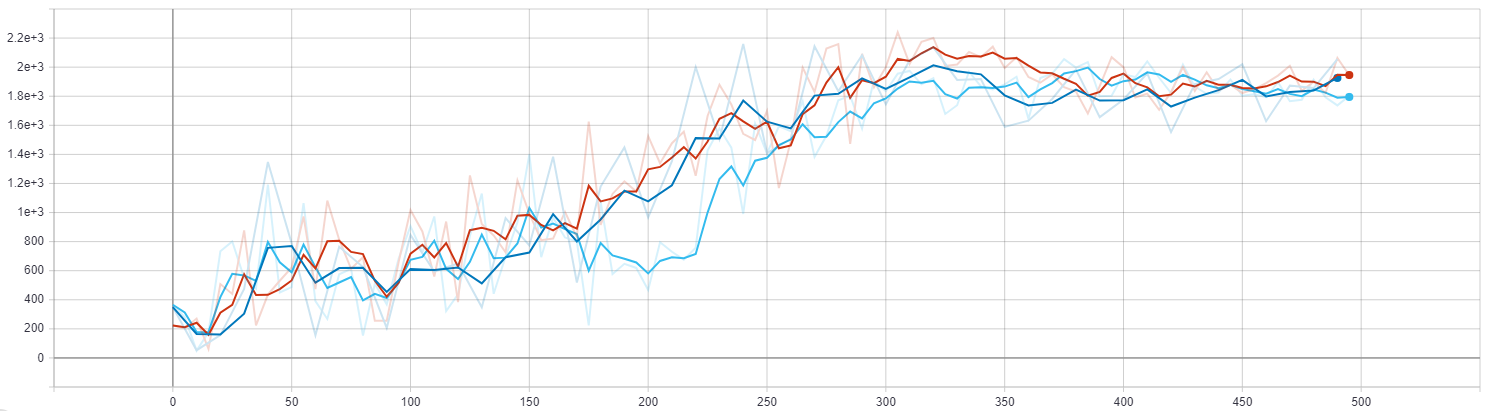
\includegraphics[width=17cm]{figures/4_test_eval_figs/algo_training_fig/num_completed_tasks.PNG}
    \caption{Number of completed tasks}
    \label{fig:algo_num_completed_tasks}
\end{figure}

\begin{figure}[h]
    \centering
    \includegraphics[width=17cm]{figures/4_test_eval_figs/algo_training_fig/num_failed_tasks.png}
    \caption{Number of failed tasks}
    \label{fig:algo_num_failed_tasks}
\end{figure}

\begin{figure}[h]
    \centering
    \includegraphics[width=17cm]{figures/4_test_eval_figs/algo_training_fig/percent_tasks.png}
    \caption{Percent of tasks attempted}
    \label{fig:algo_percent_tasks}
\end{figure}

\begin{figure}[h]
    \centering
    \includegraphics[width=17cm]{figures/4_test_eval_figs/algo_training_fig/total_prices.png}
    \caption{Total prices}
    \label{fig:algo_total_prices}
\end{figure}

\begin{figure}[h]
    \centering
    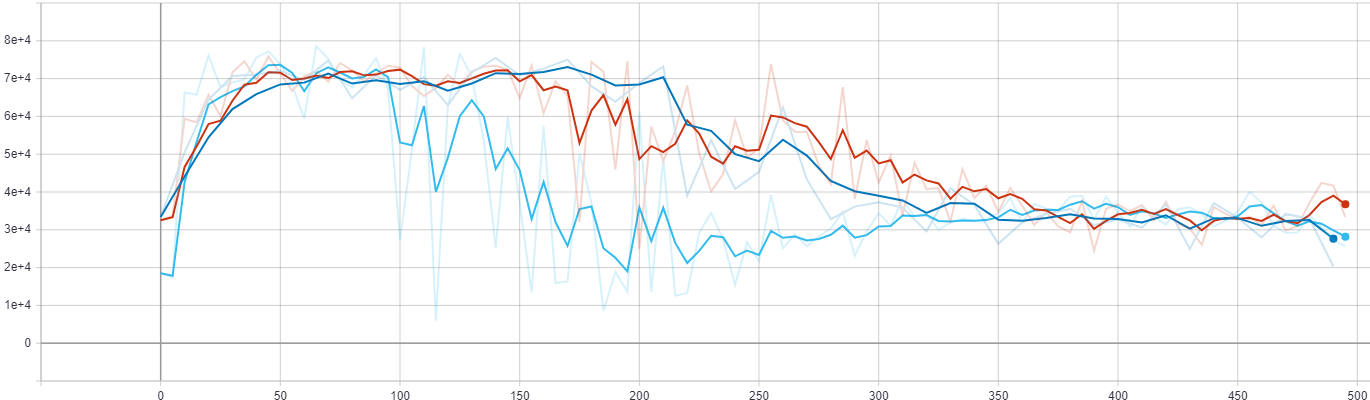
\includegraphics[width=17cm]{figures/4_test_eval_figs/algo_training_fig/total_winning_prices.PNG}
    \caption{Winning prices}
    \label{fig:algo_winning_prices}
\end{figure}

\begin{figure}[h]
    \centering
    \begin{minipage}{0.5\textwidth}
        \centering
        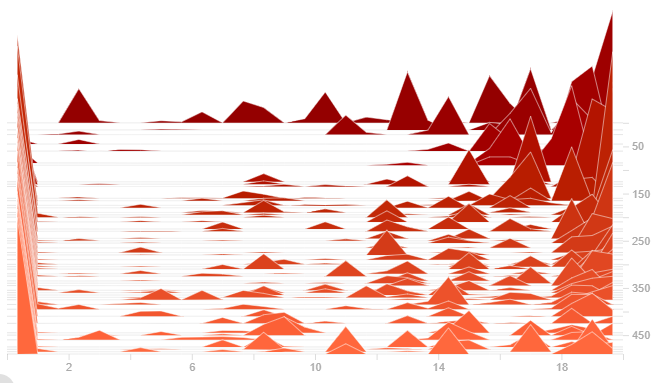
\includegraphics[width=1.0\textwidth]{figures/4_test_eval_figs/algo_training_fig/dqn_auction_prices.png}
        \caption{Deep Q Network auction prices}
        \label{fig:dqn-auction-prices}
    \end{minipage}\hfill
    \begin{minipage}{0.5\textwidth}
        \centering
        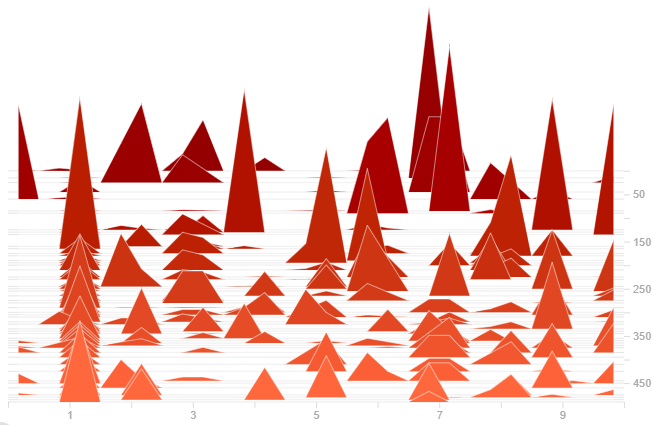
\includegraphics[width=1.0\textwidth]{figures/4_test_eval_figs/algo_training_fig/dqn_weightings.png}
        \caption{Deep Q Network resource weightings}
        \label{fig:dqn-resource-weightings}
    \end{minipage}
\end{figure}

\begin{figure}[h]
    \centering
    \begin{minipage}{0.5\textwidth}
        \centering
        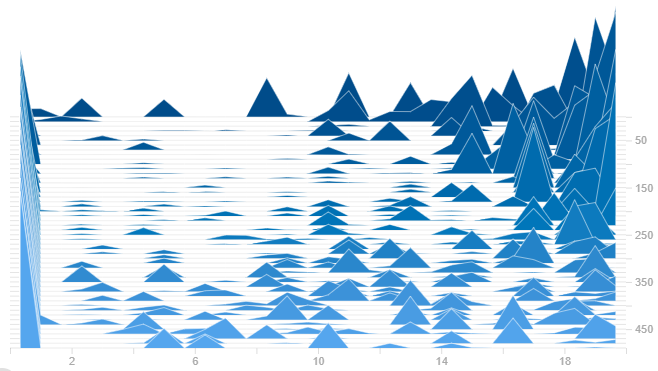
\includegraphics[width=1.0\textwidth]{figures/4_test_eval_figs/algo_training_fig/ddqn_auction_prices.png}
        \caption{Double Deep Q Network auction prices}
        \label{fig:ddqn-auction-prices}
    \end{minipage}\hfill
    \begin{minipage}{0.5\textwidth}
        \centering
        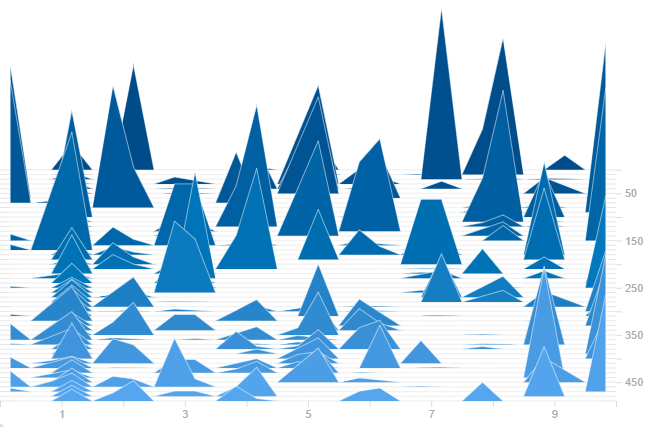
\includegraphics[width=1.0\textwidth]{figures/4_test_eval_figs/algo_training_fig/ddqn_weightings.png}
        \caption{Double Deep Q Network resource weightings}
        \label{fig:ddqn-resource-weightings}
    \end{minipage}
\end{figure}

\begin{figure}[h]
    \centering
    \begin{minipage}{0.5\textwidth}
        \centering
        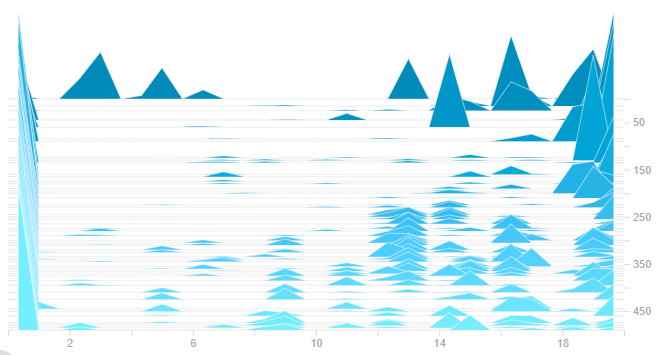
\includegraphics[width=1.0\textwidth]{figures/4_test_eval_figs/algo_training_fig/dueling_dqn_auction_prices.png}
        \caption{Dueling Deep Q Network auction prices}
        \label{fig:dueling-dqn-auction-prices}
    \end{minipage}\hfill
    \begin{minipage}{0.5\textwidth}
        \centering
        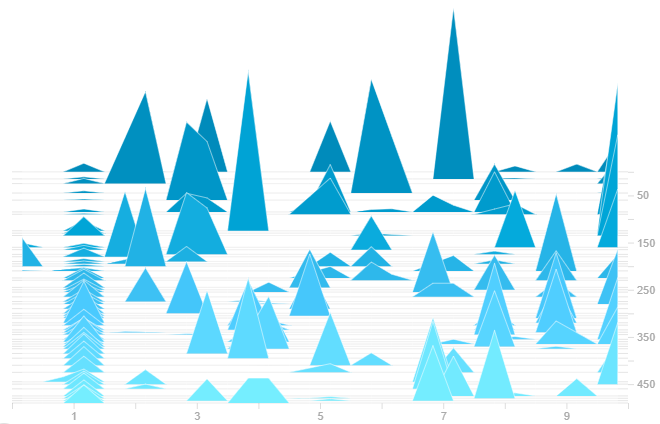
\includegraphics[width=1.0\textwidth]{figures/4_test_eval_figs/algo_training_fig/dueling_dqn_weightings.png}
        \caption{Dueling Deep Q Network resource weightings}
        \label{fig:dueling-dqn-resource-weightings}
    \end{minipage}
\end{figure}

\subsection{Neural network architecture training}\label{subsec:neural-network-architecture-training}
%% Neural network architecture testing
%% Compare architectures
There are a wide-range of compatible neural network architectures that agents can use, as outlined in
table~\ref{tab:neural_network_layers}. To use these agents, the underlying policies are kept the same with a range of
model networks are trained.

\begin{wrapfigure}{l}{0.5\textwidth}
    \includegraphics[width=0.5\textwidth]{figures/4_test_eval_figs/net_arch_training_fig/legend.png}
    \caption{Environment training legend}
    \label{fig:net-arch-training-legend}
\end{wrapfigure}

%% Training evaluation
\begin{figure}[h]
    \centering
    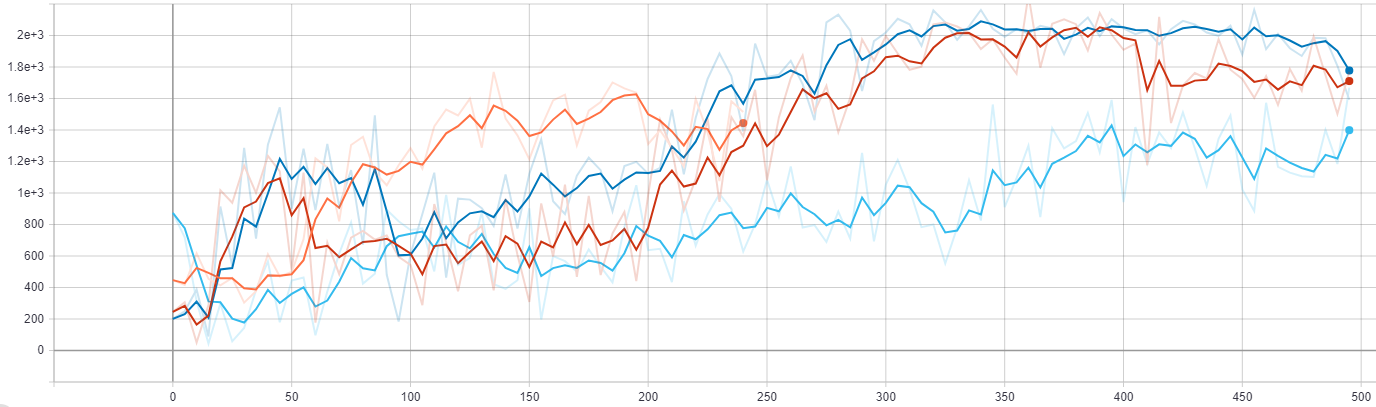
\includegraphics[width=17cm]{figures/4_test_eval_figs/net_arch_training_fig/num_completed_tasks.PNG}
    \caption{Number of completed tasks}
    \label{fig:net_arch_num_completed_tasks}
\end{figure}

\begin{figure}[h]
    \centering
    \includegraphics[width=17cm]{figures/4_test_eval_figs/net_arch_training_fig/num_failed_tasks.png}
    \caption{Number of failed tasks}
    \label{fig:net_arch_num_failed_tasks}
\end{figure}

\begin{figure}[h]
    \centering
    \includegraphics[width=17cm]{figures/4_test_eval_figs/net_arch_training_fig/percent_tasks.png}
    \caption{Percent of tasks attempted}
    \label{fig:net_arch_percent_tasks}
\end{figure}

\begin{figure}[h]
    \centering
    \includegraphics[width=17cm]{figures/4_test_eval_figs/net_arch_training_fig/total_prices.png}
    \caption{Total prices}
    \label{fig:net_arch_total_prices}
\end{figure}

\begin{figure}[h]
    \centering
    \begin{minipage}{0.5\textwidth}
        \centering
        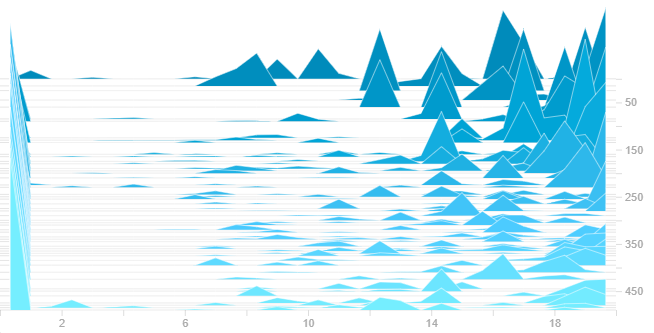
\includegraphics[width=1.0\textwidth]{figures/4_test_eval_figs/net_arch_training_fig/rnn_architecture_auction_prices.png}
        \caption{Rnn network architecture auction prices}
        \label{fig:rnn-auction-prices}
    \end{minipage}\hfill
    \begin{minipage}{0.5\textwidth}
        \centering
        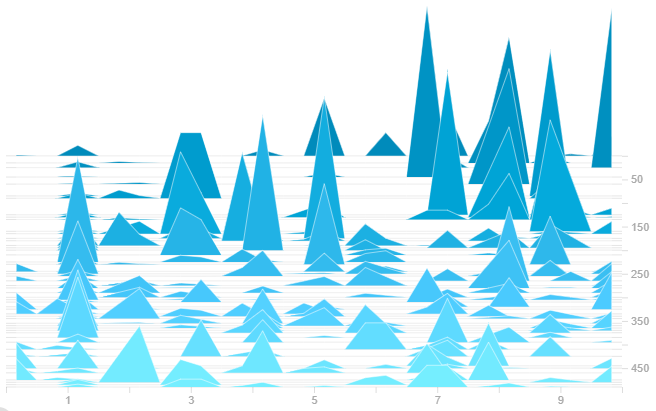
\includegraphics[width=1.0\textwidth]{figures/4_test_eval_figs/net_arch_training_fig/rnn_architecture_weightings.png}
        \caption{Rnn network architecture resource weightings}
        \label{fig:rnn-resource-weightings}
    \end{minipage}
\end{figure}

\begin{figure}[h]
    \centering
    \begin{minipage}{0.5\textwidth}
        \centering
        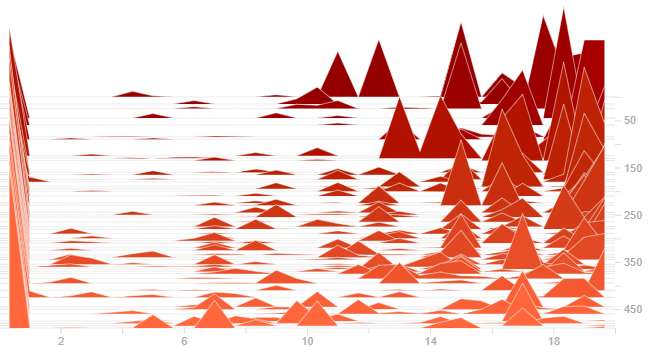
\includegraphics[width=1.0\textwidth]{figures/4_test_eval_figs/net_arch_training_fig/gru_architecture_auction_prices.png}
        \caption{GRU network architecture auction prices}
        \label{fig:gru-auction-prices}
    \end{minipage}\hfill
    \begin{minipage}{0.5\textwidth}
        \centering
        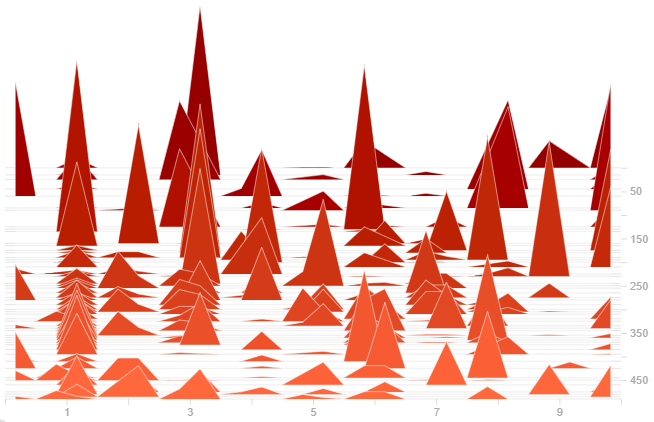
\includegraphics[width=1.0\textwidth]{figures/4_test_eval_figs/net_arch_training_fig/gru_architecture_weightings.png}
        \caption{GRU network architecture resource weightings}
        \label{fig:gru-resource-weightings}
    \end{minipage}
\end{figure}

\begin{figure}[h]
    \centering
    \begin{minipage}{0.5\textwidth}
        \centering
        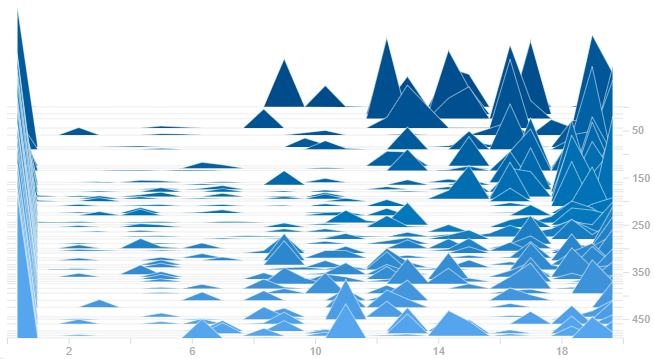
\includegraphics[width=1.0\textwidth]{figures/4_test_eval_figs/net_arch_training_fig/lstm_architecture_auction_prices.png}
        \caption{LSTM network architecture auction prices}
        \label{fig:lstm-auction-prices}
    \end{minipage}\hfill
    \begin{minipage}{0.5\textwidth}
        \centering
        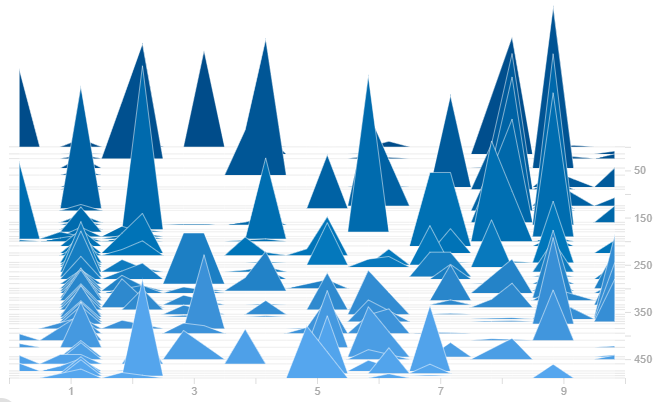
\includegraphics[width=1.0\textwidth]{figures/4_test_eval_figs/net_arch_training_fig/lstm_architecture_weightings.png}
        \caption{Rnn network architecture resource weightings}
        \label{fig:lstm-resource-weightings}
    \end{minipage}
\end{figure}

\begin{figure}[h]
    \centering
    \begin{minipage}{0.5\textwidth}
        \centering
        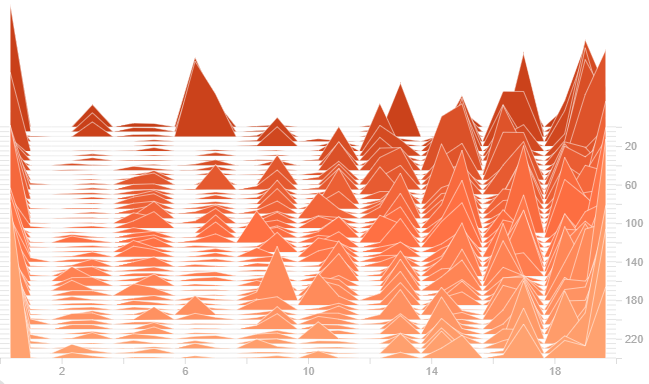
\includegraphics[width=1.0\textwidth]{figures/4_test_eval_figs/net_arch_training_fig/bidirectional_architecture_auction_prices.png}
        \caption{Bidirectional network architecture auction prices}
        \label{fig:bidirectional-auction-prices}
    \end{minipage}\hfill
    \begin{minipage}{0.5\textwidth}
        \centering
        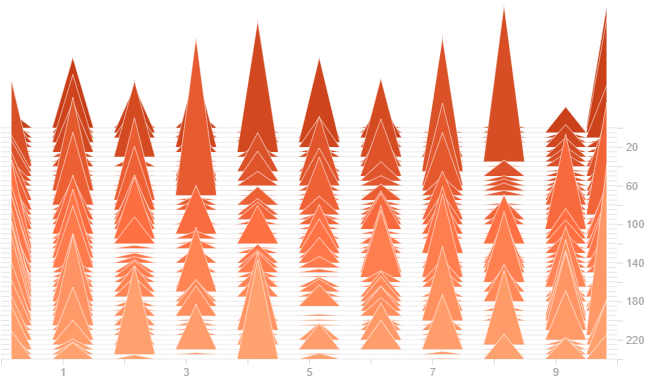
\includegraphics[width=1.0\textwidth]{figures/4_test_eval_figs/net_arch_training_fig/bidirectional_architecture_weightings.png}
        \caption{Bidirectional network architecture resource weightings}
        \label{fig:bidirectional-resource-weightings}
    \end{minipage}
\end{figure}
\chapter{Conclusion and future work}\label{ch:conclusion-and-future-work}
The aim of this project was to expand previous research to fix perceived flaws in the formulation by introducing the
notion of time into the resource allocation optimisation model. As a result, a new optimisation problem was presented
in Section~\ref{sec:optimisation-problem} with an auction mechanism proposed as well to deal with self-interested
users and to distribute tasks to self-interested servers. To know how to efficiently bid and allocation resources to
tasks, reinforcement learning agents were proposed that aimed to learn these policies. An implementation of an MEC
environment was developed and numerous reinforcement learning algorithms were used to train both auction and resource
weighting agent. These agents were found to efficiently learn an optimal policy however were found to not produce
optimal policies such that \~5\% of all tasks were no completed within there time frame. A range of reasons why this
may have occurred in Chapter~\ref{ch:testing-and-evaluation} as a well as policy gradient agents being unable to
escape local maxima prevent them from achieving results close to that of the deep Q learning agents. Therefore this
project has been viewed as a success however this author believes have more research and analysis of agents is required
before such agents can be implemented into real-life systems. \\
For future work into this project, this author believes that several additions to the agents proposed could greatly
improve their performance like n-step rewards~\citep{multi-step-dqn} and distributional agents~\citep{distributional_dqn}
that would improve Q value estimation within stochastic environment. An additional heuristic for the policy gradient,
would be use a centralised critic~\citep{maddpg} that has been proposed in mix competitive-cooperative environment to
help agents work together.


\bibliographystyle{plainnat}
\bibliography{extra/references}

\backmatter
\appendix
%! Suppress = LabelConvention
\setboolean{@twoside}{false}

\section*{Appendix A: Paper}
This paper was been produced with the authors being myself, Dr Sebastian Stein, Professor Tim Norman from Southampton
University, Dr Fidan Mehmeti, Professor Tom La Porta, Caroline Rubein from Pennsylvania State University and Dr Geeth
Demel from IBM and within this project is referred to as~\cite{FlexibleResourceAllocation}.

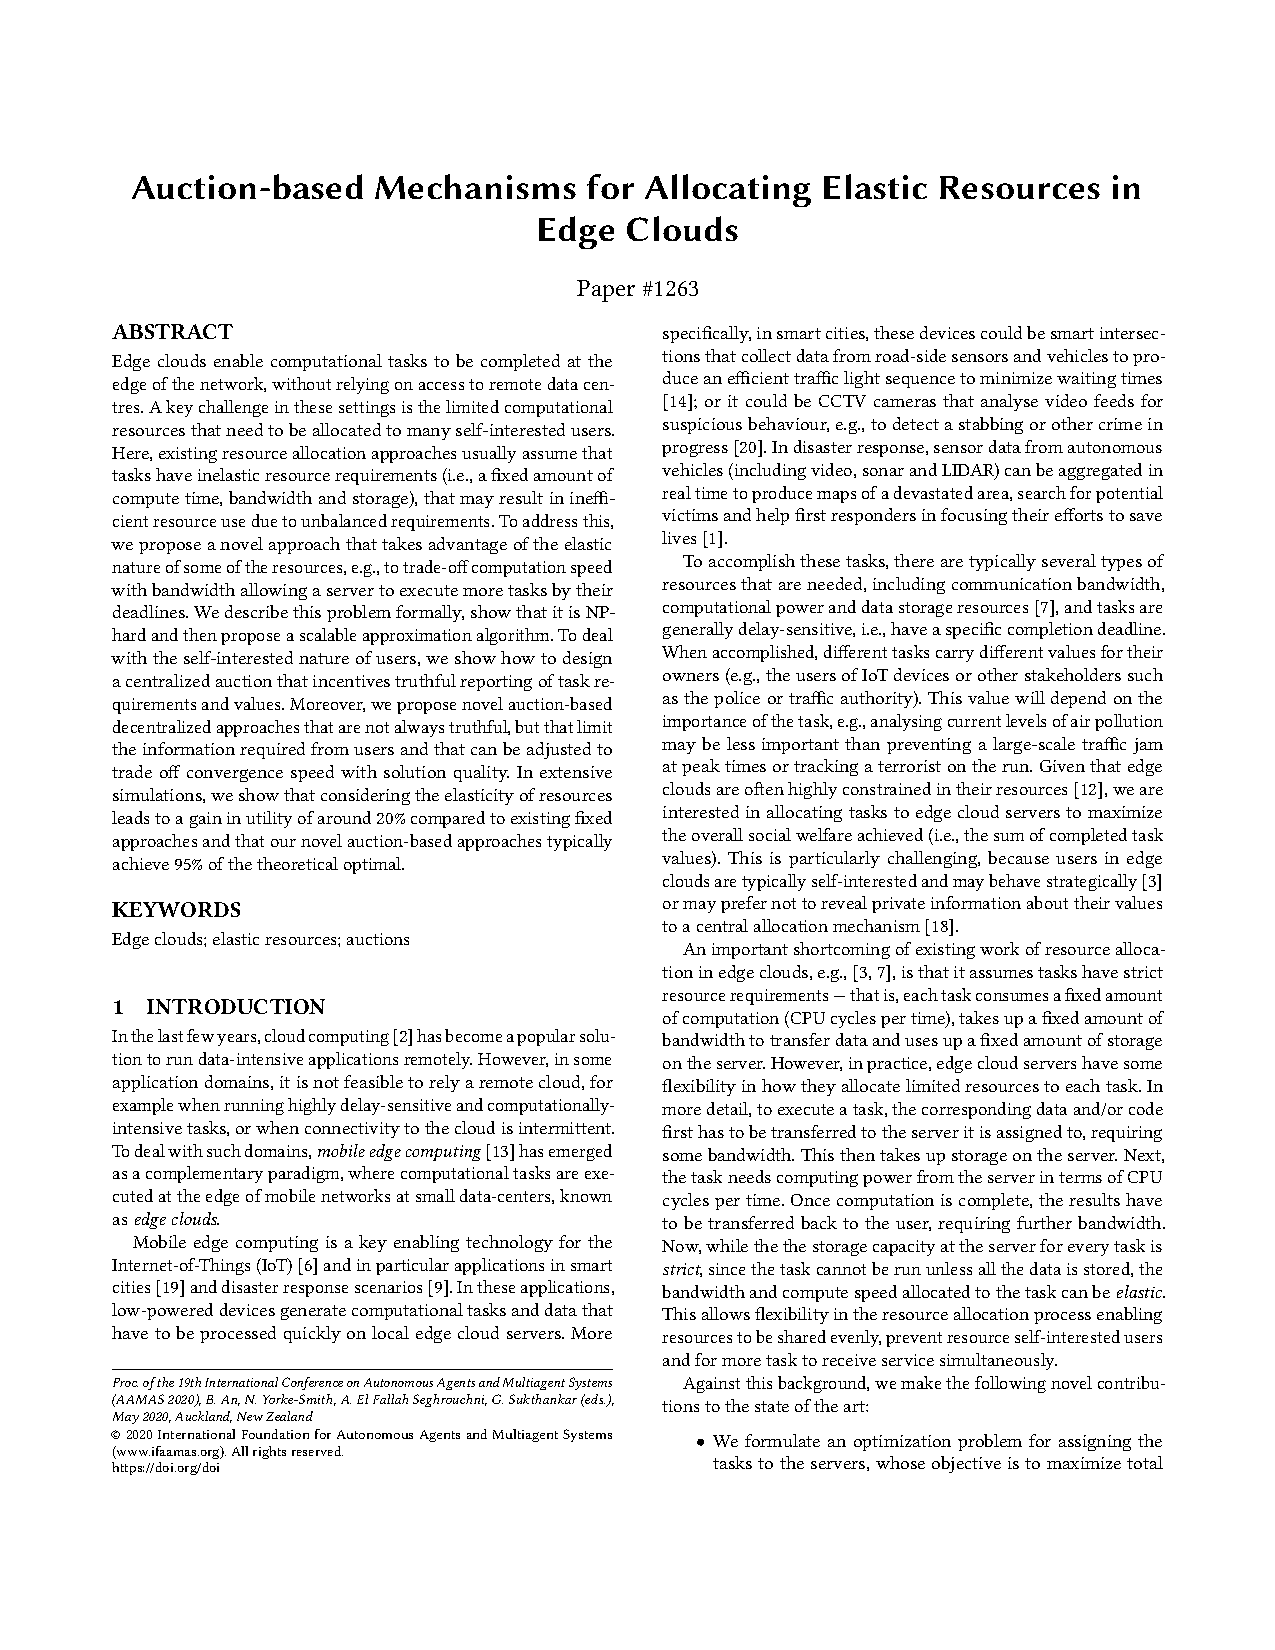
\includepdf[pages=-, offset=25mm -20mm]{extra/aamas_2020}

\section*{Appendix B: SPIE Presentation}
This presentation was produced from the same work as the~\cite{FlexibleResourceAllocation} with the title "Analytical
agility at the edge of the network through auction mechanisms" at was submitted to the conference on Artificial
Intelligence and Machine Learning for Multi-Domain Operations Applications II, as part of the SPIE Defense + Commercial
Sensing.


\includepdf[pages=-, offset=25mm -25mm, landscape=True, scale=0.95]{extra/spie_presentation}

\section*{Appendix B: Project management}
%% Risk assessment
%% Grantt chart
%%
This is the progress report submitted on the 10th of December 2019.

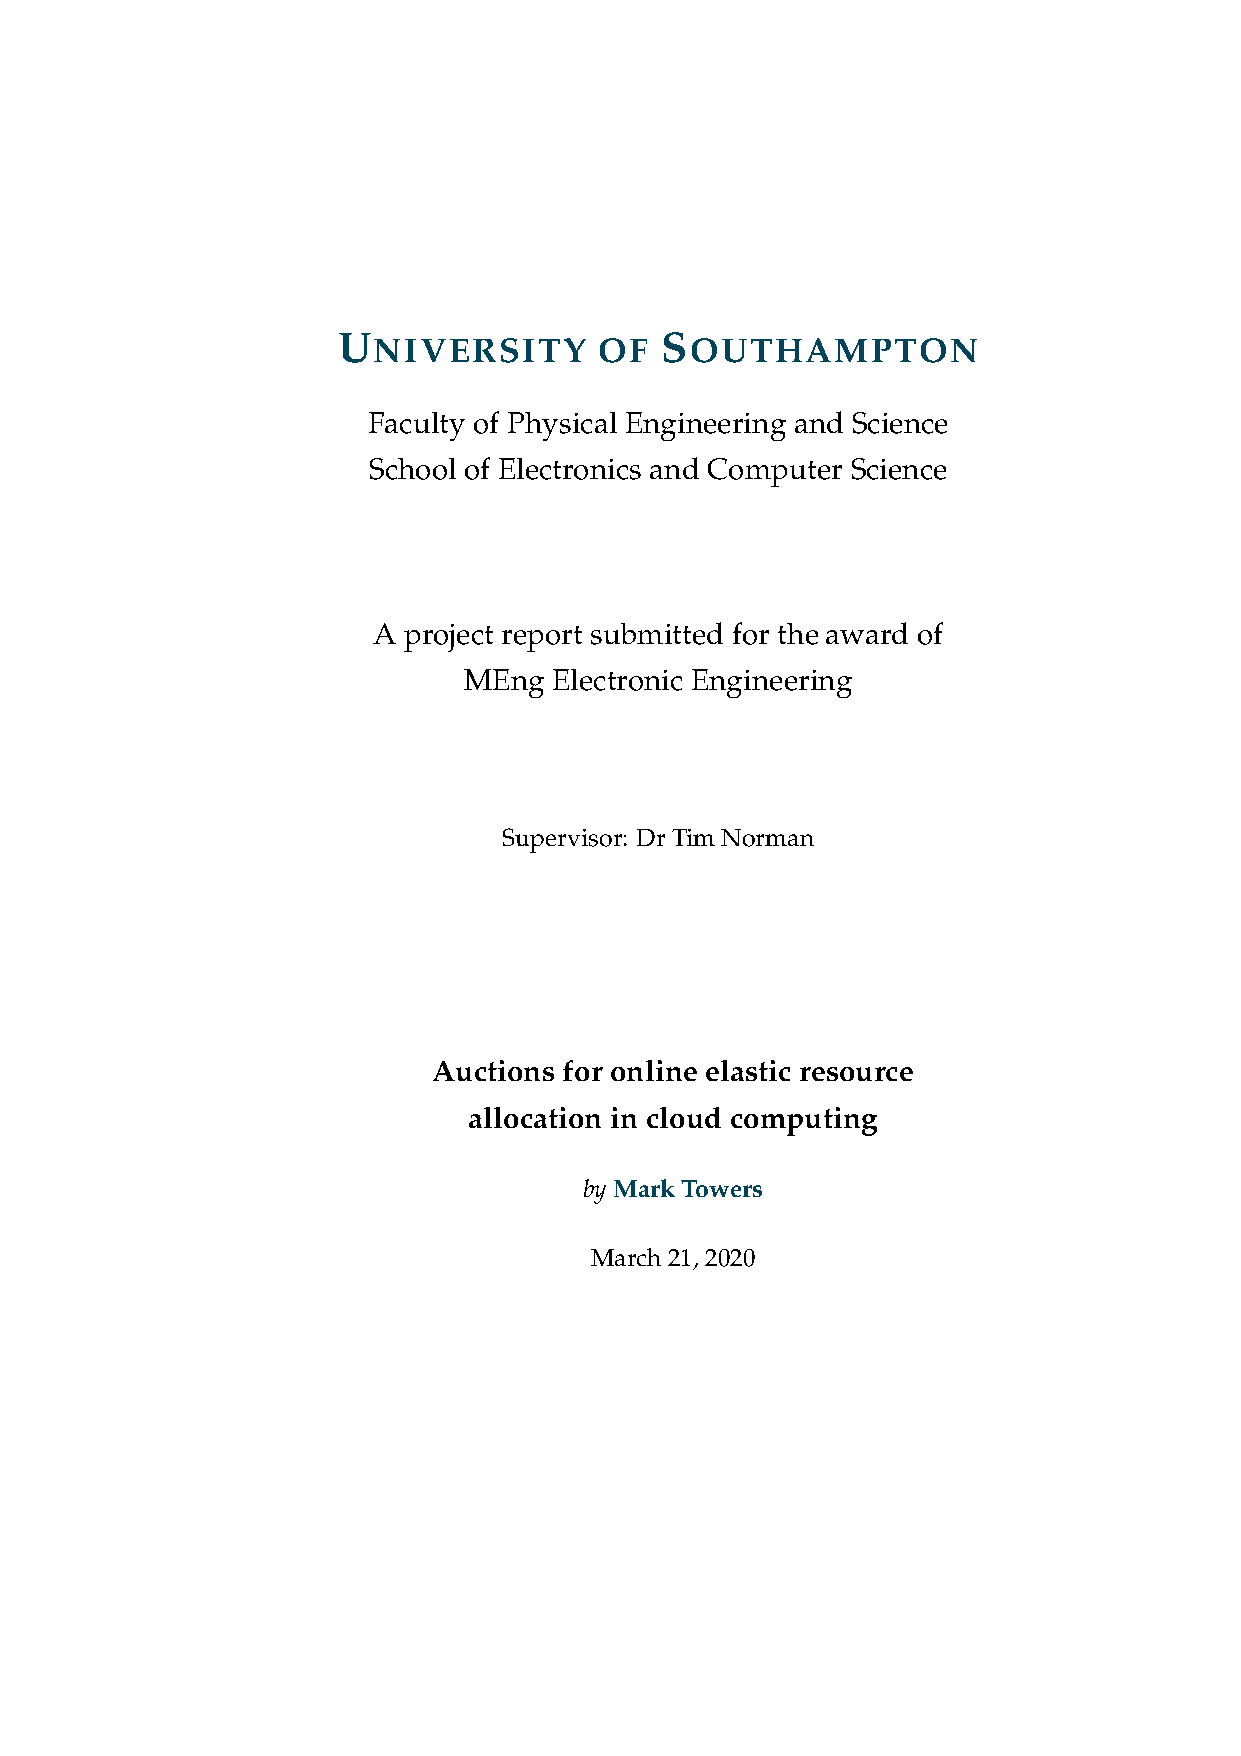
\includepdf[pages=-, offset=25mm -20mm]{extra/progress_report}


\end{document}
%% ----------------------------------------------------------------
